\documentclass[a4paper]{book}
\usepackage{a4wide}
\usepackage{makeidx}
\usepackage{fancyhdr}
\usepackage{graphicx}
\usepackage{multicol}
\usepackage{float}
\usepackage{textcomp}
\usepackage{alltt}
\usepackage[utf8]{inputenc}
\usepackage{doxygen}
\makeindex
\setcounter{tocdepth}{3}
\renewcommand{\footrulewidth}{0.4pt}
\begin{document}
\begin{titlepage}
\vspace*{7cm}
\begin{center}
{\Large OpenGLot \\[1ex]\large 0.1 }\\
\vspace*{1cm}
{\large Generated by Doxygen 1.5.8}\\
\vspace*{0.5cm}
{\small Fri Nov 20 18:09:06 2009}\\
\end{center}
\end{titlepage}
\clearemptydoublepage
\pagenumbering{roman}
\tableofcontents
\clearemptydoublepage
\pagenumbering{arabic}
\chapter{Namespace Index}
\section{Namespace List}
Here is a list of all namespaces with brief descriptions:\begin{CompactList}
\item\contentsline{section}{{\bf glot} }{\pageref{namespaceglot}}{}
\end{CompactList}

\chapter{Class Index}
\section{Class Hierarchy}
This inheritance list is sorted roughly, but not completely, alphabetically:\begin{CompactList}
\item \contentsline{section}{glot::color}{\pageref{classglot_1_1color}}{}
\item \contentsline{section}{glot::function}{\pageref{classglot_1_1function}}{}
\item \contentsline{section}{glot::grapher}{\pageref{classglot_1_1grapher}}{}
\item \contentsline{section}{glot::point}{\pageref{classglot_1_1point}}{}
\item \contentsline{section}{glot::primitive}{\pageref{classglot_1_1primitive}}{}
\begin{CompactList}
\item \contentsline{section}{glot::p\_\-curve}{\pageref{classglot_1_1p__curve}}{}
\item \contentsline{section}{glot::shader\_\-primitive}{\pageref{classglot_1_1shader__primitive}}{}
\begin{CompactList}
\item \contentsline{section}{glot::contour}{\pageref{classglot_1_1contour}}{}
\item \contentsline{section}{glot::curve}{\pageref{classglot_1_1curve}}{}
\item \contentsline{section}{glot::flow}{\pageref{classglot_1_1flow}}{}
\item \contentsline{section}{glot::scalar\_\-field}{\pageref{classglot_1_1scalar__field}}{}
\end{CompactList}
\item \contentsline{section}{glot::vector}{\pageref{classglot_1_1vector}}{}
\end{CompactList}
\item \contentsline{section}{screen}{\pageref{structscreen}}{}
\item \contentsline{section}{stopwatch}{\pageref{classstopwatch}}{}
\end{CompactList}

\chapter{Class Index}
\section{Class List}
Here are the classes, structs, unions and interfaces with brief descriptions:\begin{CompactList}
\item\contentsline{section}{{\bf glot::color} }{\pageref{classglot_1_1color}}{}
\item\contentsline{section}{{\bf glot::contour} (Curve: a \doxyref{contour}{p.}{classglot_1_1contour} to plot )}{\pageref{classglot_1_1contour}}{}
\item\contentsline{section}{{\bf glot::curve} (Curve: a \doxyref{curve}{p.}{classglot_1_1curve} to plot )}{\pageref{classglot_1_1curve}}{}
\item\contentsline{section}{{\bf glot::flow} (Flow: a vector-valued \doxyref{function}{p.}{classglot_1_1function} as a \doxyref{flow}{p.}{classglot_1_1flow} field )}{\pageref{classglot_1_1flow}}{}
\item\contentsline{section}{{\bf glot::function} }{\pageref{classglot_1_1function}}{}
\item\contentsline{section}{{\bf glot::grapher} (Grapher: an interactive plotter display )}{\pageref{classglot_1_1grapher}}{}
\item\contentsline{section}{{\bf glot::p\_\-curve} (P\_\-curve: a parametric \doxyref{curve}{p.}{classglot_1_1curve} to plot )}{\pageref{classglot_1_1p__curve}}{}
\item\contentsline{section}{{\bf glot::point} }{\pageref{classglot_1_1point}}{}
\item\contentsline{section}{{\bf glot::primitive} (Primitive: the parent class of all rendered objects )}{\pageref{classglot_1_1primitive}}{}
\item\contentsline{section}{{\bf glot::scalar\_\-field} (Scalar\_\-field: a scalar field to plot )}{\pageref{classglot_1_1scalar__field}}{}
\item\contentsline{section}{{\bf screen} }{\pageref{structscreen}}{}
\item\contentsline{section}{{\bf glot::shader\_\-primitive} (Shader\_\-primitive: the parent class of all primitives that use their own shaders )}{\pageref{classglot_1_1shader__primitive}}{}
\item\contentsline{section}{{\bf stopwatch} (Stopwatch : encapsulates timing routines )}{\pageref{classstopwatch}}{}
\item\contentsline{section}{{\bf glot::vector} }{\pageref{classglot_1_1vector}}{}
\end{CompactList}

\chapter{File Index}
\section{File List}
Here is a list of all files with brief descriptions:\begin{CompactList}
\item\contentsline{section}{{\bf color.h} }{\pageref{color_8h}}{}
\item\contentsline{section}{{\bf contour.h} }{\pageref{contour_8h}}{}
\item\contentsline{section}{{\bf curve.h} }{\pageref{curve_8h}}{}
\item\contentsline{section}{{\bf flow.h} }{\pageref{flow_8h}}{}
\item\contentsline{section}{{\bf function.h} }{\pageref{function_8h}}{}
\item\contentsline{section}{{\bf grapher.h} }{\pageref{grapher_8h}}{}
\item\contentsline{section}{{\bf p\_\-curve.h} }{\pageref{p__curve_8h}}{}
\item\contentsline{section}{{\bf point.h} }{\pageref{point_8h}}{}
\item\contentsline{section}{{\bf primitive.h} }{\pageref{primitive_8h}}{}
\item\contentsline{section}{{\bf scalar\_\-field.h} }{\pageref{scalar__field_8h}}{}
\item\contentsline{section}{{\bf screen.h} }{\pageref{screen_8h}}{}
\item\contentsline{section}{{\bf shader\_\-primitive.h} }{\pageref{shader__primitive_8h}}{}
\item\contentsline{section}{{\bf stopwatch.h} }{\pageref{stopwatch_8h}}{}
\item\contentsline{section}{{\bf vector.h} }{\pageref{vector_8h}}{}
\end{CompactList}

\chapter{Namespace Documentation}
\section{glot Namespace Reference}
\label{namespaceglot}\index{glot@{glot}}
\subsection*{Classes}
\begin{CompactItemize}
\item 
class {\bf color}
\item 
class {\bf contour}
\begin{CompactList}\small\item\em \doxyref{curve}{p.}{classglot_1_1curve}: a \doxyref{contour}{p.}{classglot_1_1contour} to plot \item\end{CompactList}\item 
class {\bf curve}
\begin{CompactList}\small\item\em \doxyref{curve}{p.}{classglot_1_1curve}: a \doxyref{curve}{p.}{classglot_1_1curve} to plot \item\end{CompactList}\item 
class {\bf flow}
\begin{CompactList}\small\item\em \doxyref{flow}{p.}{classglot_1_1flow}: a vector-valued \doxyref{function}{p.}{classglot_1_1function} as a \doxyref{flow}{p.}{classglot_1_1flow} field \item\end{CompactList}\item 
class {\bf function}
\item 
class {\bf grapher}
\begin{CompactList}\small\item\em \doxyref{grapher}{p.}{classglot_1_1grapher}: an interactive plotter display \item\end{CompactList}\item 
class {\bf p\_\-curve}
\begin{CompactList}\small\item\em \doxyref{p\_\-curve}{p.}{classglot_1_1p__curve}: a parametric \doxyref{curve}{p.}{classglot_1_1curve} to plot \item\end{CompactList}\item 
class {\bf point}
\item 
class {\bf primitive}
\begin{CompactList}\small\item\em \doxyref{primitive}{p.}{classglot_1_1primitive}: the parent class of all rendered objects \item\end{CompactList}\item 
class {\bf scalar\_\-field}
\begin{CompactList}\small\item\em \doxyref{scalar\_\-field}{p.}{classglot_1_1scalar__field}: a scalar field to plot \item\end{CompactList}\item 
class {\bf shader\_\-primitive}
\begin{CompactList}\small\item\em \doxyref{shader\_\-primitive}{p.}{classglot_1_1shader__primitive}: the parent class of all primitives that use their own shaders \item\end{CompactList}\item 
class {\bf vector}
\end{CompactItemize}
\subsection*{Enumerations}
\begin{CompactItemize}
\item 
enum {\bf display\_\-opt} \{ \par
{\bf AXES\_\-OFF} =  0, 
{\bf GRID\_\-OFF} =  0, 
{\bf X\_\-LIN} =  0, 
{\bf Y\_\-LIN} =  0, 
\par
{\bf AXES\_\-ON} =  1, 
{\bf GRID\_\-ON} =  2, 
{\bf X\_\-LOG} =  4, 
{\bf Y\_\-LOG} =  8
 \}
\begin{CompactList}\small\item\em Enumeration for display options. \item\end{CompactList}\item 
enum {\bf keyboard\_\-opt} \{ \par
{\bf ZOOM\_\-KEYS\_\-OFF} =  0, 
{\bf AXES\_\-KEYS\_\-OFF} =  0, 
{\bf GRID\_\-KEYS\_\-OFF} =  0, 
{\bf QUIT\_\-KEYS\_\-OFF} =  0, 
\par
{\bf ZOOM\_\-KEYS\_\-ON} =  1, 
{\bf AXES\_\-KEYS\_\-ON} =  2, 
{\bf GRID\_\-KEYS\_\-ON} =  4, 
{\bf QUIT\_\-KEYS\_\-ON} =  8
 \}
\begin{CompactList}\small\item\em Enumeration for keyboard action options. \item\end{CompactList}\end{CompactItemize}


\subsection{Enumeration Type Documentation}
\index{glot@{glot}!display\_\-opt@{display\_\-opt}}
\index{display\_\-opt@{display\_\-opt}!glot@{glot}}
\subsubsection[{display\_\-opt}]{\setlength{\rightskip}{0pt plus 5cm}enum {\bf glot::display\_\-opt}}\label{namespaceglot_48397641a9391dad56e97ef6699ca3e8}


Enumeration for display options. 

Bitwise or these to set the display options \begin{Desc}
\item[Enumerator: ]\par
\begin{description}
\index{AXES\_\-OFF@{AXES\_\-OFF}!glot@{glot}}\index{glot@{glot}!AXES\_\-OFF@{AXES\_\-OFF}}\item[{\em 
AXES\_\-OFF\label{namespaceglot_48397641a9391dad56e97ef6699ca3e8cc985c5059e13185b96eebc3357f1975}
}]\index{GRID\_\-OFF@{GRID\_\-OFF}!glot@{glot}}\index{glot@{glot}!GRID\_\-OFF@{GRID\_\-OFF}}\item[{\em 
GRID\_\-OFF\label{namespaceglot_48397641a9391dad56e97ef6699ca3e8f7f1a13e957aed0fed87a1ca07494c1a}
}]\index{X\_\-LIN@{X\_\-LIN}!glot@{glot}}\index{glot@{glot}!X\_\-LIN@{X\_\-LIN}}\item[{\em 
X\_\-LIN\label{namespaceglot_48397641a9391dad56e97ef6699ca3e8fe22cf1f4facde1c4647411dbf93302b}
}]\index{Y\_\-LIN@{Y\_\-LIN}!glot@{glot}}\index{glot@{glot}!Y\_\-LIN@{Y\_\-LIN}}\item[{\em 
Y\_\-LIN\label{namespaceglot_48397641a9391dad56e97ef6699ca3e8bc26e4ec70a3a053cc9537be8def5e72}
}]\index{AXES\_\-ON@{AXES\_\-ON}!glot@{glot}}\index{glot@{glot}!AXES\_\-ON@{AXES\_\-ON}}\item[{\em 
AXES\_\-ON\label{namespaceglot_48397641a9391dad56e97ef6699ca3e857ca9b6d79f02bf0970b09a1e717e457}
}]\index{GRID\_\-ON@{GRID\_\-ON}!glot@{glot}}\index{glot@{glot}!GRID\_\-ON@{GRID\_\-ON}}\item[{\em 
GRID\_\-ON\label{namespaceglot_48397641a9391dad56e97ef6699ca3e8028b91a09052eb213b4abf6283e78461}
}]\index{X\_\-LOG@{X\_\-LOG}!glot@{glot}}\index{glot@{glot}!X\_\-LOG@{X\_\-LOG}}\item[{\em 
X\_\-LOG\label{namespaceglot_48397641a9391dad56e97ef6699ca3e89ab350a7739d4dc57fff188823f098a0}
}]\index{Y\_\-LOG@{Y\_\-LOG}!glot@{glot}}\index{glot@{glot}!Y\_\-LOG@{Y\_\-LOG}}\item[{\em 
Y\_\-LOG\label{namespaceglot_48397641a9391dad56e97ef6699ca3e807f7ef89539f8db9717d4ff6a84e6385}
}]\end{description}
\end{Desc}

\index{glot@{glot}!keyboard\_\-opt@{keyboard\_\-opt}}
\index{keyboard\_\-opt@{keyboard\_\-opt}!glot@{glot}}
\subsubsection[{keyboard\_\-opt}]{\setlength{\rightskip}{0pt plus 5cm}enum {\bf glot::keyboard\_\-opt}}\label{namespaceglot_cfe91431ea4a54852a727f7834e44086}


Enumeration for keyboard action options. 

Bitwise or these to set the keyboard action options \begin{Desc}
\item[Enumerator: ]\par
\begin{description}
\index{ZOOM\_\-KEYS\_\-OFF@{ZOOM\_\-KEYS\_\-OFF}!glot@{glot}}\index{glot@{glot}!ZOOM\_\-KEYS\_\-OFF@{ZOOM\_\-KEYS\_\-OFF}}\item[{\em 
ZOOM\_\-KEYS\_\-OFF\label{namespaceglot_cfe91431ea4a54852a727f7834e4408650c81ad1bf05a21b32c0027e81bc46f4}
}]\index{AXES\_\-KEYS\_\-OFF@{AXES\_\-KEYS\_\-OFF}!glot@{glot}}\index{glot@{glot}!AXES\_\-KEYS\_\-OFF@{AXES\_\-KEYS\_\-OFF}}\item[{\em 
AXES\_\-KEYS\_\-OFF\label{namespaceglot_cfe91431ea4a54852a727f7834e44086b197d9081ff787f6c9e3b6d93cdcbace}
}]\index{GRID\_\-KEYS\_\-OFF@{GRID\_\-KEYS\_\-OFF}!glot@{glot}}\index{glot@{glot}!GRID\_\-KEYS\_\-OFF@{GRID\_\-KEYS\_\-OFF}}\item[{\em 
GRID\_\-KEYS\_\-OFF\label{namespaceglot_cfe91431ea4a54852a727f7834e4408619a13d43980e118a52f5205844003dc9}
}]\index{QUIT\_\-KEYS\_\-OFF@{QUIT\_\-KEYS\_\-OFF}!glot@{glot}}\index{glot@{glot}!QUIT\_\-KEYS\_\-OFF@{QUIT\_\-KEYS\_\-OFF}}\item[{\em 
QUIT\_\-KEYS\_\-OFF\label{namespaceglot_cfe91431ea4a54852a727f7834e44086e6d503c5f5521453adec09d665ba011c}
}]\index{ZOOM\_\-KEYS\_\-ON@{ZOOM\_\-KEYS\_\-ON}!glot@{glot}}\index{glot@{glot}!ZOOM\_\-KEYS\_\-ON@{ZOOM\_\-KEYS\_\-ON}}\item[{\em 
ZOOM\_\-KEYS\_\-ON\label{namespaceglot_cfe91431ea4a54852a727f7834e44086bc55dffb01fd33ceffe584ca30adcbab}
}]\index{AXES\_\-KEYS\_\-ON@{AXES\_\-KEYS\_\-ON}!glot@{glot}}\index{glot@{glot}!AXES\_\-KEYS\_\-ON@{AXES\_\-KEYS\_\-ON}}\item[{\em 
AXES\_\-KEYS\_\-ON\label{namespaceglot_cfe91431ea4a54852a727f7834e4408648e6d527976c5a8ba1dacea5d047f891}
}]\index{GRID\_\-KEYS\_\-ON@{GRID\_\-KEYS\_\-ON}!glot@{glot}}\index{glot@{glot}!GRID\_\-KEYS\_\-ON@{GRID\_\-KEYS\_\-ON}}\item[{\em 
GRID\_\-KEYS\_\-ON\label{namespaceglot_cfe91431ea4a54852a727f7834e440868c38cb439a3622ed773d4582272ad552}
}]\index{QUIT\_\-KEYS\_\-ON@{QUIT\_\-KEYS\_\-ON}!glot@{glot}}\index{glot@{glot}!QUIT\_\-KEYS\_\-ON@{QUIT\_\-KEYS\_\-ON}}\item[{\em 
QUIT\_\-KEYS\_\-ON\label{namespaceglot_cfe91431ea4a54852a727f7834e440860c52b21bbf99f25d58bd0ad87d32022b}
}]\end{description}
\end{Desc}


\chapter{Class Documentation}
\section{glot::color Class Reference}
\label{classglot_1_1color}\index{glot::color@{glot::color}}
{\tt \#include $<$color.h$>$}

\subsection*{Public Member Functions}
\begin{CompactItemize}
\item 
{\bf color} (double red=0, double green=0, double blue=0, double alpha=1)
\begin{CompactList}\small\item\em Constructor. \item\end{CompactList}\end{CompactItemize}
\subsection*{Public Attributes}
\begin{CompactItemize}
\item 
double {\bf r}
\begin{CompactList}\small\item\em The red component of the \doxyref{color}{p.}{classglot_1_1color}. \item\end{CompactList}\item 
double {\bf g}
\begin{CompactList}\small\item\em The green component of the \doxyref{color}{p.}{classglot_1_1color}. \item\end{CompactList}\item 
double {\bf b}
\begin{CompactList}\small\item\em The blue component of the \doxyref{color}{p.}{classglot_1_1color}. \item\end{CompactList}\item 
double {\bf a}
\begin{CompactList}\small\item\em The transparency of the \doxyref{color}{p.}{classglot_1_1color} (1 = opaque). \item\end{CompactList}\end{CompactItemize}


\subsection{Constructor \& Destructor Documentation}
\index{glot::color@{glot::color}!color@{color}}
\index{color@{color}!glot::color@{glot::color}}
\subsubsection[{color}]{\setlength{\rightskip}{0pt plus 5cm}glot::color::color (double {\em red} = {\tt 0}, \/  double {\em green} = {\tt 0}, \/  double {\em blue} = {\tt 0}, \/  double {\em alpha} = {\tt 1})\hspace{0.3cm}{\tt  [inline]}}\label{classglot_1_1color_aa1bd417bdab7b47076fbde85ccb2ba9}


Constructor. 

\begin{Desc}
\item[Parameters:]
\begin{description}
\item[{\em red}]- red component of \doxyref{color}{p.}{classglot_1_1color} \item[{\em green}]- green component of \doxyref{color}{p.}{classglot_1_1color} \item[{\em blue}]- blue component of \doxyref{color}{p.}{classglot_1_1color} \item[{\em alpha}]- the transparency of the \doxyref{color}{p.}{classglot_1_1color} \end{description}
\end{Desc}


\subsection{Member Data Documentation}
\index{glot::color@{glot::color}!a@{a}}
\index{a@{a}!glot::color@{glot::color}}
\subsubsection[{a}]{\setlength{\rightskip}{0pt plus 5cm}double {\bf glot::color::a}}\label{classglot_1_1color_c47e5ca02bf2a171e22607409740f827}


The transparency of the \doxyref{color}{p.}{classglot_1_1color} (1 = opaque). 

\index{glot::color@{glot::color}!b@{b}}
\index{b@{b}!glot::color@{glot::color}}
\subsubsection[{b}]{\setlength{\rightskip}{0pt plus 5cm}double {\bf glot::color::b}}\label{classglot_1_1color_638f4163ecba1d756c4bde06acc81aa8}


The blue component of the \doxyref{color}{p.}{classglot_1_1color}. 

\index{glot::color@{glot::color}!g@{g}}
\index{g@{g}!glot::color@{glot::color}}
\subsubsection[{g}]{\setlength{\rightskip}{0pt plus 5cm}double {\bf glot::color::g}}\label{classglot_1_1color_c1cfcfb1ee54d040ab03dc7d952b3ab4}


The green component of the \doxyref{color}{p.}{classglot_1_1color}. 

\index{glot::color@{glot::color}!r@{r}}
\index{r@{r}!glot::color@{glot::color}}
\subsubsection[{r}]{\setlength{\rightskip}{0pt plus 5cm}double {\bf glot::color::r}}\label{classglot_1_1color_fce286e75c4e917163ff02e38f6163c8}


The red component of the \doxyref{color}{p.}{classglot_1_1color}. 



The documentation for this class was generated from the following file:\begin{CompactItemize}
\item 
{\bf color.h}\end{CompactItemize}

\section{glot::contour Class Reference}
\label{classglot_1_1contour}\index{glot::contour@{glot::contour}}
\doxyref{curve}{p.}{classglot_1_1curve}: a \doxyref{contour}{p.}{classglot_1_1contour} to plot  


{\tt \#include $<$contour.h$>$}

Inheritance diagram for glot::contour::\begin{figure}[H]
\begin{center}
\leavevmode
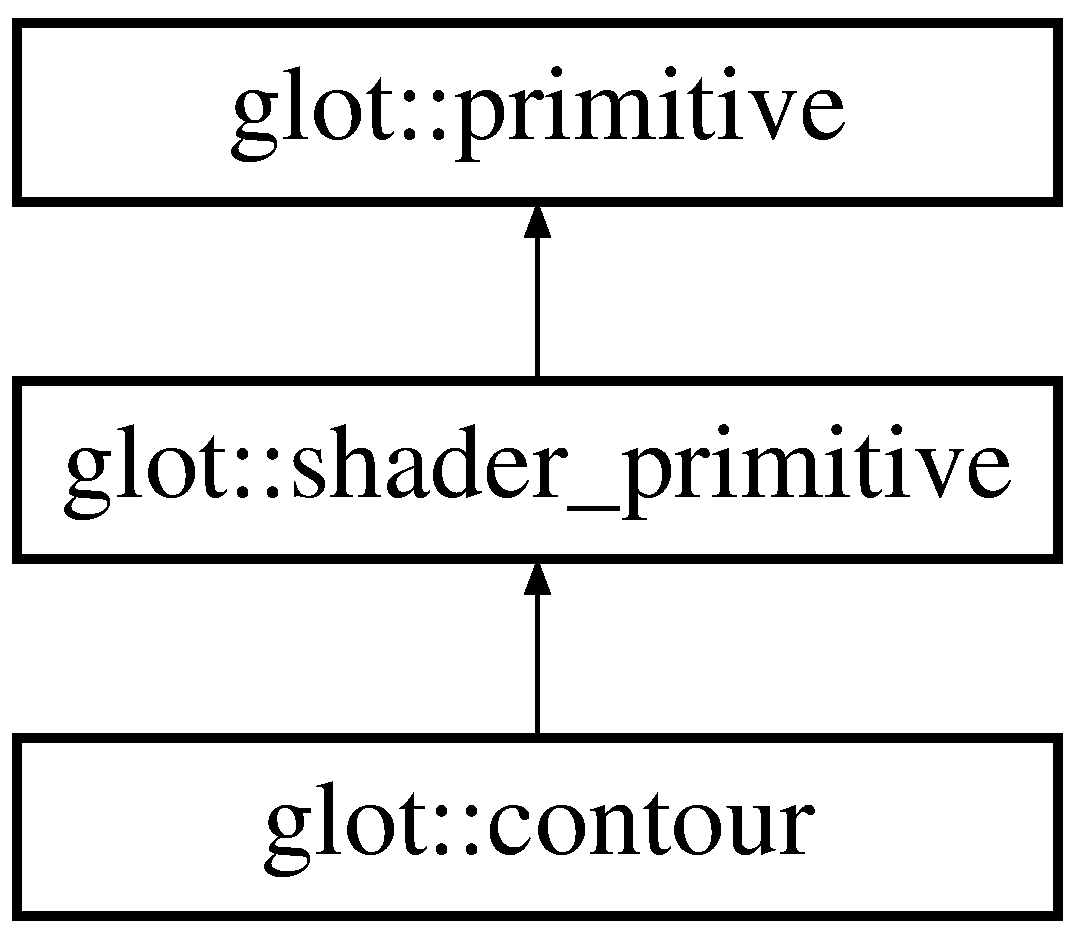
\includegraphics[height=3cm]{classglot_1_1contour}
\end{center}
\end{figure}
\subsection*{Public Member Functions}
\begin{CompactItemize}
\item 
{\bf contour} (const string \&{\bf f}, const {\bf color} \&col)
\begin{CompactList}\small\item\em Constructor. \item\end{CompactList}\item 
void {\bf dl\_\-gen} (const {\bf screen} \&scr)
\begin{CompactList}\small\item\em Display-list generator. \item\end{CompactList}\end{CompactItemize}


\subsection{Detailed Description}
\doxyref{curve}{p.}{classglot_1_1curve}: a \doxyref{contour}{p.}{classglot_1_1contour} to plot 

This class maps a scalar \doxyref{function}{p.}{classglot_1_1function} of two variables to a 2-d plot showing the iso-curve z = 0

\begin{Desc}
\item[See also:]\doxyref{grapher}{p.}{classglot_1_1grapher} \end{Desc}


\subsection{Constructor \& Destructor Documentation}
\index{glot::contour@{glot::contour}!contour@{contour}}
\index{contour@{contour}!glot::contour@{glot::contour}}
\subsubsection[{contour}]{\setlength{\rightskip}{0pt plus 5cm}glot::contour::contour (const string \& {\em f}, \/  const {\bf color} \& {\em col})\hspace{0.3cm}{\tt  [inline]}}\label{classglot_1_1contour_c2efb4c4edc6a8b9c7f4572148e1684d}


Constructor. 

\begin{Desc}
\item[Parameters:]
\begin{description}
\item[{\em f}]- A \doxyref{function}{p.}{classglot_1_1function} of x, y and t \item[{\em col}]- the \doxyref{color}{p.}{classglot_1_1color} of the \doxyref{curve}{p.}{classglot_1_1curve}\end{description}
\end{Desc}
The \doxyref{function}{p.}{classglot_1_1function} may use x, y and t and any combination of C-available functions. Rather, any C-available functions supported by the OpenGL Shading Language (GLSL) which includes most.

NOTE: GLSL is very picky about typecasting. When using integer values use the float equivalent instead: (Use 1.0 not 1, 93.0 not 93) 

\subsection{Member Function Documentation}
\index{glot::contour@{glot::contour}!dl\_\-gen@{dl\_\-gen}}
\index{dl\_\-gen@{dl\_\-gen}!glot::contour@{glot::contour}}
\subsubsection[{dl\_\-gen}]{\setlength{\rightskip}{0pt plus 5cm}void glot::contour::dl\_\-gen (const {\bf screen} \& {\em scr})\hspace{0.3cm}{\tt  [virtual]}}\label{classglot_1_1contour_ad1f9a15676372dfb398e68772f59625}


Display-list generator. 

\begin{Desc}
\item[Parameters:]
\begin{description}
\item[{\em scr}]- The specifications of the \doxyref{screen}{p.}{structscreen}\end{description}
\end{Desc}
This returns the geometry appropriate for the geometry shader used here. In this case, it's a set of line segments that specify a bounding square for which the shader should find the iso-curve. That is, a line from (x\_\-min, y\_\-min) to (x\_\-max, y\_\-max) 

Implements {\bf glot::primitive} \doxyref{}{p.}{classglot_1_1primitive_2e8c612e7642561ae3536a865c08a436}.

The documentation for this class was generated from the following file:\begin{CompactItemize}
\item 
{\bf contour.h}\end{CompactItemize}

\section{glot::curve Class Reference}
\label{classglot_1_1curve}\index{glot::curve@{glot::curve}}
\doxyref{curve}{p.}{classglot_1_1curve}: a \doxyref{curve}{p.}{classglot_1_1curve} to plot  


{\tt \#include $<$curve.h$>$}

Inheritance diagram for glot::curve::\begin{figure}[H]
\begin{center}
\leavevmode
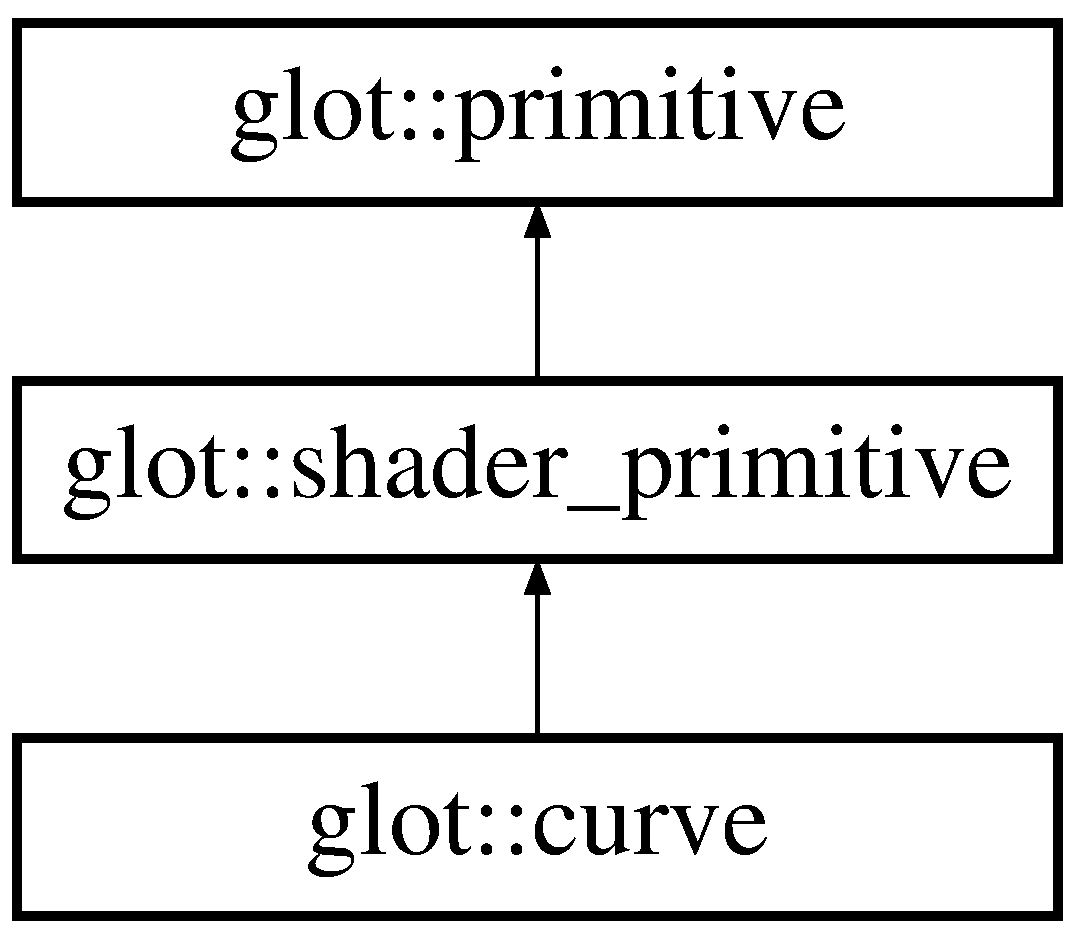
\includegraphics[height=3cm]{classglot_1_1curve}
\end{center}
\end{figure}
\subsection*{Public Member Functions}
\begin{CompactItemize}
\item 
{\bf curve} (string f, const {\bf color} \&col)
\begin{CompactList}\small\item\em Constructor. \item\end{CompactList}\item 
void {\bf dl\_\-gen} (const {\bf screen} \&s)
\begin{CompactList}\small\item\em Display-list generator. \item\end{CompactList}\end{CompactItemize}
\subsection*{Public Attributes}
\begin{CompactItemize}
\item 
{\bf color} {\bf c}
\begin{CompactList}\small\item\em Color variable. \item\end{CompactList}\end{CompactItemize}


\subsection{Detailed Description}
\doxyref{curve}{p.}{classglot_1_1curve}: a \doxyref{curve}{p.}{classglot_1_1curve} to plot 

This class takes a \doxyref{function}{p.}{classglot_1_1function} that accepts a double and returns a double and does its best to plot it in the \doxyref{grapher}{p.}{classglot_1_1grapher}.

\begin{Desc}
\item[See also:]\doxyref{grapher}{p.}{classglot_1_1grapher} 

\doxyref{p\_\-curve}{p.}{classglot_1_1p__curve} \end{Desc}


\subsection{Constructor \& Destructor Documentation}
\index{glot::curve@{glot::curve}!curve@{curve}}
\index{curve@{curve}!glot::curve@{glot::curve}}
\subsubsection[{curve}]{\setlength{\rightskip}{0pt plus 5cm}glot::curve::curve (string {\em f}, \/  const {\bf color} \& {\em col})\hspace{0.3cm}{\tt  [inline]}}\label{classglot_1_1curve_07edcd368d122ad3585eef52e3775c4e}


Constructor. 

\begin{Desc}
\item[Parameters:]
\begin{description}
\item[{\em func}]- the \doxyref{function}{p.}{classglot_1_1function} to render \item[{\em col}]- the \doxyref{color}{p.}{classglot_1_1color} of the \doxyref{curve}{p.}{classglot_1_1curve} \end{description}
\end{Desc}


\subsection{Member Function Documentation}
\index{glot::curve@{glot::curve}!dl\_\-gen@{dl\_\-gen}}
\index{dl\_\-gen@{dl\_\-gen}!glot::curve@{glot::curve}}
\subsubsection[{dl\_\-gen}]{\setlength{\rightskip}{0pt plus 5cm}void glot::curve::dl\_\-gen (const {\bf screen} \& {\em s})\hspace{0.3cm}{\tt  [virtual]}}\label{classglot_1_1curve_29cf8bdce745306212af7c147023fba4}


Display-list generator. 

\begin{Desc}
\item[Parameters:]
\begin{description}
\item[{\em s}]- the \doxyref{screen}{p.}{structscreen} specs\end{description}
\end{Desc}
The \doxyref{screen}{p.}{structscreen} stores the dimensions of the plot, etc. and based on that information, this \doxyref{function}{p.}{classglot_1_1function} generates the geometry for the \doxyref{primitive}{p.}{classglot_1_1primitive}. Typically this might be stored in a display list, but that is up to the container class, \doxyref{grapher}{p.}{classglot_1_1grapher} 

Implements {\bf glot::primitive} \doxyref{}{p.}{classglot_1_1primitive_2e8c612e7642561ae3536a865c08a436}.

\subsection{Member Data Documentation}
\index{glot::curve@{glot::curve}!c@{c}}
\index{c@{c}!glot::curve@{glot::curve}}
\subsubsection[{c}]{\setlength{\rightskip}{0pt plus 5cm}{\bf color} {\bf glot::curve::c}}\label{classglot_1_1curve_fcd83ec8bb2dbcb8b148a192f0a9c99b}


Color variable. 

This is the \doxyref{color}{p.}{classglot_1_1color} the \doxyref{curve}{p.}{classglot_1_1curve} is supposed to take on. 

Reimplemented from {\bf glot::primitive} \doxyref{}{p.}{classglot_1_1primitive_ea0f7ab17148686a80fb68230eb09eba}.

The documentation for this class was generated from the following file:\begin{CompactItemize}
\item 
{\bf curve.h}\end{CompactItemize}

\section{glot::flow Class Reference}
\label{classglot_1_1flow}\index{glot::flow@{glot::flow}}
\doxyref{flow}{p.}{classglot_1_1flow}: a vector-valued \doxyref{function}{p.}{classglot_1_1function} as a \doxyref{flow}{p.}{classglot_1_1flow} field  


{\tt \#include $<$flow.h$>$}

Inheritance diagram for glot::flow::\begin{figure}[H]
\begin{center}
\leavevmode
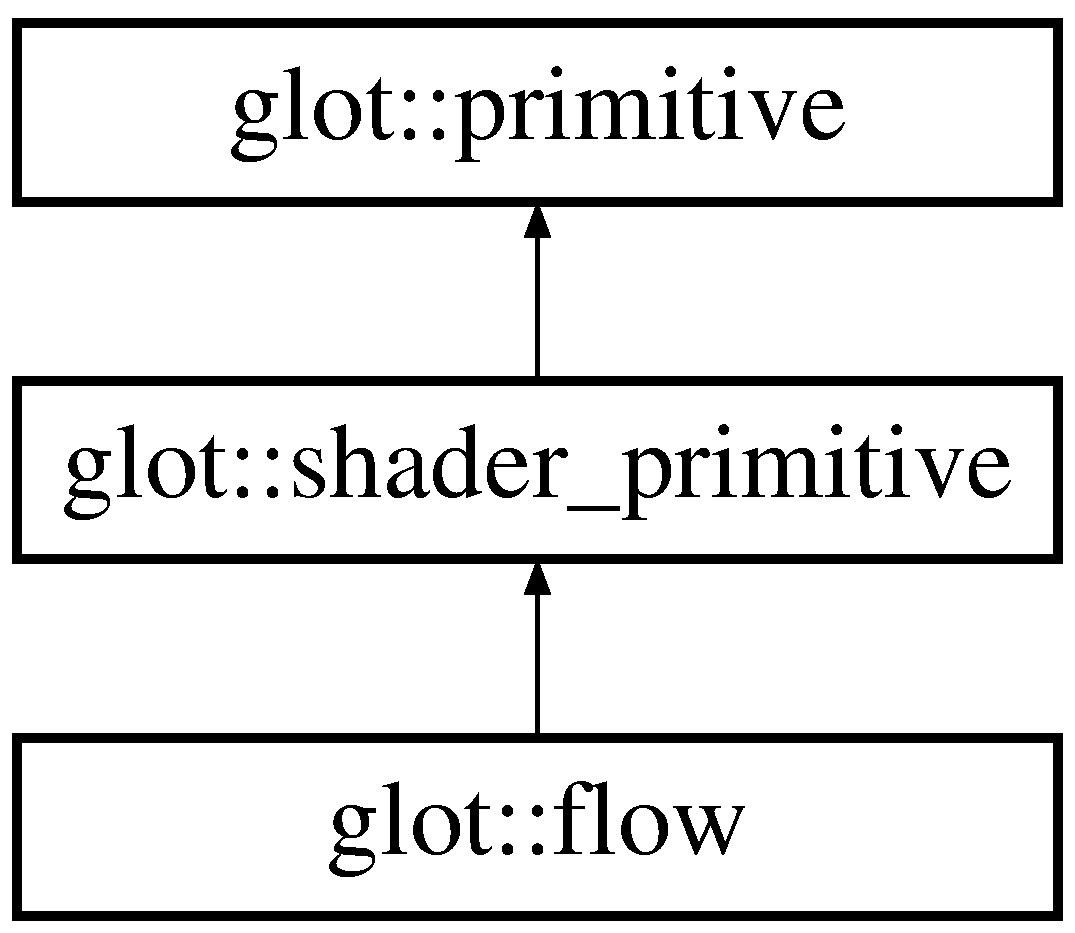
\includegraphics[height=3cm]{classglot_1_1flow}
\end{center}
\end{figure}
\subsection*{Public Member Functions}
\begin{CompactItemize}
\item 
{\bf flow} (const string \&{\bf f})
\begin{CompactList}\small\item\em Constructor. \item\end{CompactList}\item 
void {\bf dl\_\-gen} (const {\bf screen} \&scr)
\begin{CompactList}\small\item\em Display-list generator. \item\end{CompactList}\end{CompactItemize}


\subsection{Detailed Description}
\doxyref{flow}{p.}{classglot_1_1flow}: a vector-valued \doxyref{function}{p.}{classglot_1_1function} as a \doxyref{flow}{p.}{classglot_1_1flow} field 

This class represents a vector-valued \doxyref{function}{p.}{classglot_1_1function} of x, y and t as a \doxyref{flow}{p.}{classglot_1_1flow} field using streamlines. It uses fourth-order Runge-Kutta integration to determine the next points in the line, and along the line linearly increases the alpha value. This is contrary to the ink smearing analogy, and more the comet tail analogy (in ink smearing the tail points forward, and in the comet analogy the tail points backwards). 

\subsection{Constructor \& Destructor Documentation}
\index{glot::flow@{glot::flow}!flow@{flow}}
\index{flow@{flow}!glot::flow@{glot::flow}}
\subsubsection[{flow}]{\setlength{\rightskip}{0pt plus 5cm}glot::flow::flow (const string \& {\em f})\hspace{0.3cm}{\tt  [inline]}}\label{classglot_1_1flow_c4b04c5c286ea1616afdb3579a5983a5}


Constructor. 

\begin{Desc}
\item[Parameters:]
\begin{description}
\item[{\em func}]- the vector-valued \doxyref{function}{p.}{classglot_1_1function} to render \end{description}
\end{Desc}


\subsection{Member Function Documentation}
\index{glot::flow@{glot::flow}!dl\_\-gen@{dl\_\-gen}}
\index{dl\_\-gen@{dl\_\-gen}!glot::flow@{glot::flow}}
\subsubsection[{dl\_\-gen}]{\setlength{\rightskip}{0pt plus 5cm}void glot::flow::dl\_\-gen (const {\bf screen} \& {\em scr})\hspace{0.3cm}{\tt  [virtual]}}\label{classglot_1_1flow_9b7fb4fd93ca8b9938b65e5810e4b596}


Display-list generator. 

\begin{Desc}
\item[Parameters:]
\begin{description}
\item[{\em scr}]- the \doxyref{screen}{p.}{structscreen} specs of the plot\end{description}
\end{Desc}
This \doxyref{function}{p.}{classglot_1_1function} generates the geometry that the geometry shader expects (a set of seed points). They are uniformly spaced on a grid. 

Implements {\bf glot::primitive} \doxyref{}{p.}{classglot_1_1primitive_2e8c612e7642561ae3536a865c08a436}.

The documentation for this class was generated from the following file:\begin{CompactItemize}
\item 
{\bf flow.h}\end{CompactItemize}

\section{glot::function Class Reference}
\label{classglot_1_1function}\index{glot::function@{glot::function}}
{\tt \#include $<$function.h$>$}

\subsection*{Public Types}
\begin{CompactItemize}
\item 
typedef double($\ast$ {\bf double\_\-function} )(double x)
\begin{CompactList}\small\item\em A double-to-double mapping. \item\end{CompactList}\item 
typedef double($\ast$ {\bf double\_\-2d\_\-1d\_\-function} )(double x, double y)
\begin{CompactList}\small\item\em A 2D to 1D mapping \doxyref{function}{p.}{classglot_1_1function}. \item\end{CompactList}\end{CompactItemize}
\subsection*{Public Member Functions}
\begin{CompactItemize}
\item 
{\bf function} ({\bf double\_\-function} f)
\begin{CompactList}\small\item\em Constructor. \item\end{CompactList}\item 
{\bf function} ({\bf double\_\-2d\_\-1d\_\-function} f)
\item 
double {\bf eval} (double x) const 
\begin{CompactList}\small\item\em Evaluate the \doxyref{function}{p.}{classglot_1_1function} at a \doxyref{point}{p.}{classglot_1_1point}. \item\end{CompactList}\item 
double {\bf eval} (double x, double y) const 
\end{CompactItemize}


\subsection{Member Typedef Documentation}
\index{glot::function@{glot::function}!double\_\-2d\_\-1d\_\-function@{double\_\-2d\_\-1d\_\-function}}
\index{double\_\-2d\_\-1d\_\-function@{double\_\-2d\_\-1d\_\-function}!glot::function@{glot::function}}
\subsubsection[{double\_\-2d\_\-1d\_\-function}]{\setlength{\rightskip}{0pt plus 5cm}typedef double($\ast$ {\bf glot::function::double\_\-2d\_\-1d\_\-function})(double x, double y)}\label{classglot_1_1function_91d4be64f7117589838ac0b3fe9b23b1}


A 2D to 1D mapping \doxyref{function}{p.}{classglot_1_1function}. 

\begin{Desc}
\item[Parameters:]
\begin{description}
\item[{\em x}]- the x parameter \item[{\em y}]- the y parameter \end{description}
\end{Desc}
\index{glot::function@{glot::function}!double\_\-function@{double\_\-function}}
\index{double\_\-function@{double\_\-function}!glot::function@{glot::function}}
\subsubsection[{double\_\-function}]{\setlength{\rightskip}{0pt plus 5cm}typedef double($\ast$ {\bf glot::function::double\_\-function})(double x)}\label{classglot_1_1function_3f6044874b0c63c9e94fdfc9efdc3c0f}


A double-to-double mapping. 

\begin{Desc}
\item[Parameters:]
\begin{description}
\item[{\em x}]- for a given x, return another double\end{description}
\end{Desc}
Just a mapping of R1 onto R1, using any C++ code meeting that definition 

\subsection{Constructor \& Destructor Documentation}
\index{glot::function@{glot::function}!function@{function}}
\index{function@{function}!glot::function@{glot::function}}
\subsubsection[{function}]{\setlength{\rightskip}{0pt plus 5cm}glot::function::function ({\bf double\_\-function} {\em f})\hspace{0.3cm}{\tt  [inline]}}\label{classglot_1_1function_a64607fe978be9a1bb7755f7b3e7ec77}


Constructor. 

\begin{Desc}
\item[Parameters:]
\begin{description}
\item[{\em f}]- a \doxyref{function}{p.}{classglot_1_1function} \end{description}
\end{Desc}
\index{glot::function@{glot::function}!function@{function}}
\index{function@{function}!glot::function@{glot::function}}
\subsubsection[{function}]{\setlength{\rightskip}{0pt plus 5cm}glot::function::function ({\bf double\_\-2d\_\-1d\_\-function} {\em f})\hspace{0.3cm}{\tt  [inline]}}\label{classglot_1_1function_7f68aea2102bedbf8bd767a2f9f0fe84}




\subsection{Member Function Documentation}
\index{glot::function@{glot::function}!eval@{eval}}
\index{eval@{eval}!glot::function@{glot::function}}
\subsubsection[{eval}]{\setlength{\rightskip}{0pt plus 5cm}double glot::function::eval (double {\em x}, \/  double {\em y}) const\hspace{0.3cm}{\tt  [inline]}}\label{classglot_1_1function_d7f50ab65cf1a71769e11685cc5e10ea}


\index{glot::function@{glot::function}!eval@{eval}}
\index{eval@{eval}!glot::function@{glot::function}}
\subsubsection[{eval}]{\setlength{\rightskip}{0pt plus 5cm}double glot::function::eval (double {\em x}) const\hspace{0.3cm}{\tt  [inline]}}\label{classglot_1_1function_a4ba49f5a09aa9c64b44e708d3839af9}


Evaluate the \doxyref{function}{p.}{classglot_1_1function} at a \doxyref{point}{p.}{classglot_1_1point}. 

\begin{Desc}
\item[Parameters:]
\begin{description}
\item[{\em x}]- the x value at which to evaluate \end{description}
\end{Desc}


The documentation for this class was generated from the following file:\begin{CompactItemize}
\item 
{\bf function.h}\end{CompactItemize}

\section{glot::grapher Class Reference}
\label{classglot_1_1grapher}\index{glot::grapher@{glot::grapher}}
\doxyref{grapher}{p.}{classglot_1_1grapher}: an interactive plotter display  


{\tt \#include $<$grapher.h$>$}

\subsection*{Public Types}
\begin{CompactItemize}
\item 
typedef void($\ast$ {\bf keyboard\_\-function} )(unsigned char key, GLint x, GLint y)
\begin{CompactList}\small\item\em Keyboard event handler typedef. \item\end{CompactList}\item 
typedef void($\ast$ {\bf click\_\-function} )(GLint button, GLint x, GLint y)
\begin{CompactList}\small\item\em Click even handler typedef. \item\end{CompactList}\item 
typedef void($\ast$ {\bf idle\_\-function} )(void)
\begin{CompactList}\small\item\em The idle \doxyref{function}{p.}{classglot_1_1function} typedef. \item\end{CompactList}\end{CompactItemize}
\subsection*{Static Public Member Functions}
\begin{CompactItemize}
\item 
static int {\bf initialize} (int argc, char $\ast$$\ast$argv, short int options=AXES\_\-ON$|$GRID\_\-ON$|$X\_\-LIN$|$Y\_\-LIN, short int k\_\-options=ZOOM\_\-KEYS\_\-ON$|$AXES\_\-KEYS\_\-ON$|$GRID\_\-KEYS\_\-ON$|$QUIT\_\-KEYS\_\-ON)
\begin{CompactList}\small\item\em Initialize the \doxyref{grapher}{p.}{classglot_1_1grapher}. \item\end{CompactList}\item 
static void {\bf run} ()
\begin{CompactList}\small\item\em Enter the OpenGL main loop after initialization. \item\end{CompactList}\item 
static void {\bf redraw} ()
\begin{CompactList}\small\item\em User-requested redraw. \item\end{CompactList}\item 
static void {\bf add} ({\bf primitive} \&p)
\begin{CompactList}\small\item\em Add a \doxyref{primitive}{p.}{classglot_1_1primitive} to the plot. \item\end{CompactList}\item 
static void {\bf remove} ({\bf primitive} \&p)
\begin{CompactList}\small\item\em Remove a \doxyref{primitive}{p.}{classglot_1_1primitive} from the plot. \item\end{CompactList}\item 
static void {\bf add} ({\bf point} \&p)
\begin{CompactList}\small\item\em Add a \doxyref{point}{p.}{classglot_1_1point} to the plot. \item\end{CompactList}\item 
static void {\bf remove} ({\bf point} \&p)
\begin{CompactList}\small\item\em Remove a \doxyref{point}{p.}{classglot_1_1point} from the plot. \item\end{CompactList}\item 
static void {\bf set\_\-keyboard\_\-function} ({\bf keyboard\_\-function} k)
\begin{CompactList}\small\item\em Set up a keyboard event handler. \item\end{CompactList}\item 
static void {\bf set\_\-click\_\-function} ({\bf click\_\-function} c)
\begin{CompactList}\small\item\em Set up a click event handler. \item\end{CompactList}\item 
static void {\bf set\_\-idle\_\-function} ({\bf idle\_\-function} i)
\begin{CompactList}\small\item\em Set the idle \doxyref{function}{p.}{classglot_1_1function} handler. \item\end{CompactList}\item 
static void {\bf zoom} (double scale)
\begin{CompactList}\small\item\em Zoom in / out by a scale. \item\end{CompactList}\item 
static double {\bf get\_\-x\_\-coord} (GLint x)
\begin{CompactList}\small\item\em Transform a \doxyref{screen}{p.}{structscreen} x coordinate to a world one. \item\end{CompactList}\item 
static double {\bf get\_\-y\_\-coord} (GLint y)
\begin{CompactList}\small\item\em Transform a \doxyref{screen}{p.}{structscreen} y coordinate to a world one. \item\end{CompactList}\item 
static {\bf point} {\bf get\_\-point} (GLint x, GLint y)
\begin{CompactList}\small\item\em Returns the x, y \doxyref{point}{p.}{classglot_1_1point} clicked on, in plot-space. \item\end{CompactList}\end{CompactItemize}


\subsection{Detailed Description}
\doxyref{grapher}{p.}{classglot_1_1grapher}: an interactive plotter display 

You might think of this class as a container for all the graphing primitives you plan to plot

\begin{Desc}
\item[See also:]\doxyref{p\_\-curve}{p.}{classglot_1_1p__curve} 

\doxyref{point}{p.}{classglot_1_1point} 

\doxyref{curve}{p.}{classglot_1_1curve} \end{Desc}


\subsection{Member Typedef Documentation}
\index{glot::grapher@{glot::grapher}!click\_\-function@{click\_\-function}}
\index{click\_\-function@{click\_\-function}!glot::grapher@{glot::grapher}}
\subsubsection[{click\_\-function}]{\setlength{\rightskip}{0pt plus 5cm}typedef void($\ast$ {\bf glot::grapher::click\_\-function})(GLint button, GLint x, GLint y)}\label{classglot_1_1grapher_c945e6ebe60c3cfeb0b8768c19a4d5c5}


Click even handler typedef. 

\begin{Desc}
\item[Parameters:]
\begin{description}
\item[{\em button}]- GLint button pressed \item[{\em x}]- GLint x coordinate \item[{\em y}]- GLint y coordinate\end{description}
\end{Desc}
See set\_\-click\_\-function(...) for more details \index{glot::grapher@{glot::grapher}!idle\_\-function@{idle\_\-function}}
\index{idle\_\-function@{idle\_\-function}!glot::grapher@{glot::grapher}}
\subsubsection[{idle\_\-function}]{\setlength{\rightskip}{0pt plus 5cm}typedef void($\ast$ {\bf glot::grapher::idle\_\-function})(void)}\label{classglot_1_1grapher_c7676ae32ea15cf6e1a14b4d89279740}


The idle \doxyref{function}{p.}{classglot_1_1function} typedef. 

See set\_\-idle\_\-funciton(...) for more details \index{glot::grapher@{glot::grapher}!keyboard\_\-function@{keyboard\_\-function}}
\index{keyboard\_\-function@{keyboard\_\-function}!glot::grapher@{glot::grapher}}
\subsubsection[{keyboard\_\-function}]{\setlength{\rightskip}{0pt plus 5cm}typedef void($\ast$ {\bf glot::grapher::keyboard\_\-function})(unsigned char key, GLint x, GLint y)}\label{classglot_1_1grapher_e11b07f266aff004839c7558599ce34d}


Keyboard event handler typedef. 

\begin{Desc}
\item[Parameters:]
\begin{description}
\item[{\em key}]- unsigned char \item[{\em x}]- GLint x coordinate \item[{\em y}]- GLint y coordinate\end{description}
\end{Desc}
A keyboard event handler accepts a key and x, y coordinates 

\subsection{Member Function Documentation}
\index{glot::grapher@{glot::grapher}!add@{add}}
\index{add@{add}!glot::grapher@{glot::grapher}}
\subsubsection[{add}]{\setlength{\rightskip}{0pt plus 5cm}static void glot::grapher::add ({\bf point} \& {\em p})\hspace{0.3cm}{\tt  [static]}}\label{classglot_1_1grapher_755971f366a8598dd27e720ffe8e077d}


Add a \doxyref{point}{p.}{classglot_1_1point} to the plot. 

\begin{Desc}
\item[Parameters:]
\begin{description}
\item[{\em p}]- The Point you wish to add to the plot\end{description}
\end{Desc}
Instantiate a \doxyref{point}{p.}{classglot_1_1point} and then add it to the plot with this \doxyref{function}{p.}{classglot_1_1function}. NOTE: Does not automatically request a redisplay \index{glot::grapher@{glot::grapher}!add@{add}}
\index{add@{add}!glot::grapher@{glot::grapher}}
\subsubsection[{add}]{\setlength{\rightskip}{0pt plus 5cm}static void glot::grapher::add ({\bf primitive} \& {\em p})\hspace{0.3cm}{\tt  [static]}}\label{classglot_1_1grapher_3f3e39caee2ec38dc9c21d6d3c9ed564}


Add a \doxyref{primitive}{p.}{classglot_1_1primitive} to the plot. 

\begin{Desc}
\item[Parameters:]
\begin{description}
\item[{\em p}]- the \doxyref{primitive}{p.}{classglot_1_1primitive} to add\end{description}
\end{Desc}
Add any \doxyref{primitive}{p.}{classglot_1_1primitive} that inherits from the \doxyref{primitive}{p.}{classglot_1_1primitive} class to the plot. The only requirement is that dl\_\-gen makes the required OpenGL calls to render the geometry. \index{glot::grapher@{glot::grapher}!get\_\-point@{get\_\-point}}
\index{get\_\-point@{get\_\-point}!glot::grapher@{glot::grapher}}
\subsubsection[{get\_\-point}]{\setlength{\rightskip}{0pt plus 5cm}static {\bf point} glot::grapher::get\_\-point (GLint {\em x}, \/  GLint {\em y})\hspace{0.3cm}{\tt  [static]}}\label{classglot_1_1grapher_b9ab1757f92269b3f34c47e0ef5881ea}


Returns the x, y \doxyref{point}{p.}{classglot_1_1point} clicked on, in plot-space. 

Deprecation likely \index{glot::grapher@{glot::grapher}!get\_\-x\_\-coord@{get\_\-x\_\-coord}}
\index{get\_\-x\_\-coord@{get\_\-x\_\-coord}!glot::grapher@{glot::grapher}}
\subsubsection[{get\_\-x\_\-coord}]{\setlength{\rightskip}{0pt plus 5cm}static double glot::grapher::get\_\-x\_\-coord (GLint {\em x})\hspace{0.3cm}{\tt  [static]}}\label{classglot_1_1grapher_28eb9d91df1a3fcfbbae75800311c5e5}


Transform a \doxyref{screen}{p.}{structscreen} x coordinate to a world one. 

\begin{Desc}
\item[Parameters:]
\begin{description}
\item[{\em x}]- the \doxyref{screen}{p.}{structscreen} x coordinate to transform\end{description}
\end{Desc}
It's the grapher's responsibility to know how to transform a \doxyref{screen}{p.}{structscreen} coordinate into a world coordinate with this \doxyref{function}{p.}{classglot_1_1function}. \index{glot::grapher@{glot::grapher}!get\_\-y\_\-coord@{get\_\-y\_\-coord}}
\index{get\_\-y\_\-coord@{get\_\-y\_\-coord}!glot::grapher@{glot::grapher}}
\subsubsection[{get\_\-y\_\-coord}]{\setlength{\rightskip}{0pt plus 5cm}static double glot::grapher::get\_\-y\_\-coord (GLint {\em y})\hspace{0.3cm}{\tt  [static]}}\label{classglot_1_1grapher_51de9f9fe8d7febf52b3eb02803df8bd}


Transform a \doxyref{screen}{p.}{structscreen} y coordinate to a world one. 

\begin{Desc}
\item[Parameters:]
\begin{description}
\item[{\em y}]- the \doxyref{screen}{p.}{structscreen} y coordinate to transform\end{description}
\end{Desc}
It's the grapher's repsonsibility to know how to transform a \doxyref{screen}{p.}{structscreen} coordinate into a world coordinate with this \doxyref{function}{p.}{classglot_1_1function}. \index{glot::grapher@{glot::grapher}!initialize@{initialize}}
\index{initialize@{initialize}!glot::grapher@{glot::grapher}}
\subsubsection[{initialize}]{\setlength{\rightskip}{0pt plus 5cm}static int glot::grapher::initialize (int {\em argc}, \/  char $\ast$$\ast$ {\em argv}, \/  short int {\em options} = {\tt AXES\_\-ON$|$GRID\_\-ON$|$X\_\-LIN$|$Y\_\-LIN}, \/  short int {\em k\_\-options} = {\tt ZOOM\_\-KEYS\_\-ON$|$AXES\_\-KEYS\_\-ON$|$GRID\_\-KEYS\_\-ON$|$QUIT\_\-KEYS\_\-ON})\hspace{0.3cm}{\tt  [static]}}\label{classglot_1_1grapher_820bee383b1d8d4540377f38755c4b37}


Initialize the \doxyref{grapher}{p.}{classglot_1_1grapher}. 

\begin{Desc}
\item[Parameters:]
\begin{description}
\item[{\em argc}]- same as argc used for OpenGL initialization \item[{\em argv}]- same as argv used for OpenGL initialization \item[{\em options}]- startup options \item[{\em k\_\-options}]- the default keyboard actions options\end{description}
\end{Desc}
Use a bitwise or to select startup options: AXES\_\-ON, AXES\_\-OFF GRID\_\-ON, GRID\_\-OFF X\_\-LIN, X\_\-LOG (linear x scale or logarithmic) Y\_\-LIN, Y\_\-LOG (linear y scale or logarithmic) \index{glot::grapher@{glot::grapher}!redraw@{redraw}}
\index{redraw@{redraw}!glot::grapher@{glot::grapher}}
\subsubsection[{redraw}]{\setlength{\rightskip}{0pt plus 5cm}static void glot::grapher::redraw ()\hspace{0.3cm}{\tt  [static]}}\label{classglot_1_1grapher_3059b797e6369454e302840427cf1056}


User-requested redraw. 

If you create an event handler that will make some changes to the graph, you can make those changes and then request a redraw with this \doxyref{function}{p.}{classglot_1_1function}. \index{glot::grapher@{glot::grapher}!remove@{remove}}
\index{remove@{remove}!glot::grapher@{glot::grapher}}
\subsubsection[{remove}]{\setlength{\rightskip}{0pt plus 5cm}static void glot::grapher::remove ({\bf point} \& {\em p})\hspace{0.3cm}{\tt  [static]}}\label{classglot_1_1grapher_b21410f759afb3ecfc8e2c74ff732532}


Remove a \doxyref{point}{p.}{classglot_1_1point} from the plot. 

\begin{Desc}
\item[Parameters:]
\begin{description}
\item[{\em p}]- The \doxyref{point}{p.}{classglot_1_1point} you wish to remove from the plot\end{description}
\end{Desc}
If you've plotted a \doxyref{point}{p.}{classglot_1_1point}, you can remove it from the plot with this \doxyref{function}{p.}{classglot_1_1function}. NOTE: Does not automatically request a redisplay. \index{glot::grapher@{glot::grapher}!remove@{remove}}
\index{remove@{remove}!glot::grapher@{glot::grapher}}
\subsubsection[{remove}]{\setlength{\rightskip}{0pt plus 5cm}static void glot::grapher::remove ({\bf primitive} \& {\em p})\hspace{0.3cm}{\tt  [static]}}\label{classglot_1_1grapher_2a89eb6c69bc5101896a050edc5f9e4b}


Remove a \doxyref{primitive}{p.}{classglot_1_1primitive} from the plot. 

\begin{Desc}
\item[Parameters:]
\begin{description}
\item[{\em p}]- the \doxyref{primitive}{p.}{classglot_1_1primitive} to remove\end{description}
\end{Desc}
Remove a previously-added \doxyref{primitive}{p.}{classglot_1_1primitive} from the plot \index{glot::grapher@{glot::grapher}!run@{run}}
\index{run@{run}!glot::grapher@{glot::grapher}}
\subsubsection[{run}]{\setlength{\rightskip}{0pt plus 5cm}static void glot::grapher::run ()\hspace{0.3cm}{\tt  [static]}}\label{classglot_1_1grapher_0b2131ed9108518ec725887e4ab6d857}


Enter the OpenGL main loop after initialization. 

In general, you will set up your event handlers, main code, etc., and then when you've gotten everything in place, you call \doxyref{grapher::run()}{p.}{classglot_1_1grapher_0b2131ed9108518ec725887e4ab6d857} to start the program's OpenGL portion. \index{glot::grapher@{glot::grapher}!set\_\-click\_\-function@{set\_\-click\_\-function}}
\index{set\_\-click\_\-function@{set\_\-click\_\-function}!glot::grapher@{glot::grapher}}
\subsubsection[{set\_\-click\_\-function}]{\setlength{\rightskip}{0pt plus 5cm}static void glot::grapher::set\_\-click\_\-function ({\bf click\_\-function} {\em c})\hspace{0.3cm}{\tt  [static]}}\label{classglot_1_1grapher_8f231e0cc424ff02fd27140483b8bd6a}


Set up a click event handler. 

\begin{Desc}
\item[Parameters:]
\begin{description}
\item[{\em c}]- the \doxyref{function}{p.}{classglot_1_1function} you'd like to handle click events\end{description}
\end{Desc}
If you'd like to set up a \doxyref{function}{p.}{classglot_1_1function} to handle click events (which are when a user presses down and then releases a button at the same spot), you can register it with this \doxyref{function}{p.}{classglot_1_1function}. NOTE: this is different from a motion \doxyref{function}{p.}{classglot_1_1function}. \index{glot::grapher@{glot::grapher}!set\_\-idle\_\-function@{set\_\-idle\_\-function}}
\index{set\_\-idle\_\-function@{set\_\-idle\_\-function}!glot::grapher@{glot::grapher}}
\subsubsection[{set\_\-idle\_\-function}]{\setlength{\rightskip}{0pt plus 5cm}static void glot::grapher::set\_\-idle\_\-function ({\bf idle\_\-function} {\em i})\hspace{0.3cm}{\tt  [static]}}\label{classglot_1_1grapher_23c90782ec374fe9b45fb24c6ce09c32}


Set the idle \doxyref{function}{p.}{classglot_1_1function} handler. 

Animation is done by setting the idle\_\-function handler, and this provides the interface. This might be deprecated in favor of an option that just allows the user to turn on animation, which would consist of simply setting OpenGL's idle \doxyref{function}{p.}{classglot_1_1function} to grapher's display \doxyref{function}{p.}{classglot_1_1function}. \index{glot::grapher@{glot::grapher}!set\_\-keyboard\_\-function@{set\_\-keyboard\_\-function}}
\index{set\_\-keyboard\_\-function@{set\_\-keyboard\_\-function}!glot::grapher@{glot::grapher}}
\subsubsection[{set\_\-keyboard\_\-function}]{\setlength{\rightskip}{0pt plus 5cm}static void glot::grapher::set\_\-keyboard\_\-function ({\bf keyboard\_\-function} {\em k})\hspace{0.3cm}{\tt  [static]}}\label{classglot_1_1grapher_363838298e124cc4424c5a9ccf22baf9}


Set up a keyboard event handler. 

\begin{Desc}
\item[Parameters:]
\begin{description}
\item[{\em k}]- the \doxyref{function}{p.}{classglot_1_1function} you'd like to handle key events\end{description}
\end{Desc}
If you'd like to set up a \doxyref{function}{p.}{classglot_1_1function} to handle key events, you can register them with this \doxyref{function}{p.}{classglot_1_1function}. NOTE: there are default behaviors for certain keys that are not overridden here. For example, '+' zooms in, but if you use that key as well, both a zoom and your operation will take place.

The idea behind this is that these default behaviors are not the programmer's responsibility to code up as well. They are interface freebies.

Bitwise or options together from the set: ZOOM\_\-KEYS\_\-ON / ZOOM\_\-KEYS\_\-OFF AXES\_\-KEYS\_\-ON / AXES\_\-KEYS\_\-OFF GRID\_\-KEYS\_\-ON / GRID\_\-KEYS\_\-OFF \index{glot::grapher@{glot::grapher}!zoom@{zoom}}
\index{zoom@{zoom}!glot::grapher@{glot::grapher}}
\subsubsection[{zoom}]{\setlength{\rightskip}{0pt plus 5cm}static void glot::grapher::zoom (double {\em scale})\hspace{0.3cm}{\tt  [static]}}\label{classglot_1_1grapher_b5a455dd251b5fb6e2035d014fd4bdd9}


Zoom in / out by a scale. 

\begin{Desc}
\item[Parameters:]
\begin{description}
\item[{\em scale}]- the scale by which to zoom\end{description}
\end{Desc}
This determines the center of the plot as it is now, and scales in / out by a factor of scale outward / inward from that center \doxyref{point}{p.}{classglot_1_1point}. 

The documentation for this class was generated from the following file:\begin{CompactItemize}
\item 
{\bf grapher.h}\end{CompactItemize}

\section{glot::p\_\-curve Class Reference}
\label{classglot_1_1p__curve}\index{glot::p\_\-curve@{glot::p\_\-curve}}
\doxyref{p\_\-curve}{p.}{classglot_1_1p__curve}: a parametric \doxyref{curve}{p.}{classglot_1_1curve} to plot  


{\tt \#include $<$p\_\-curve.h$>$}

Inheritance diagram for glot::p\_\-curve::\begin{figure}[H]
\begin{center}
\leavevmode
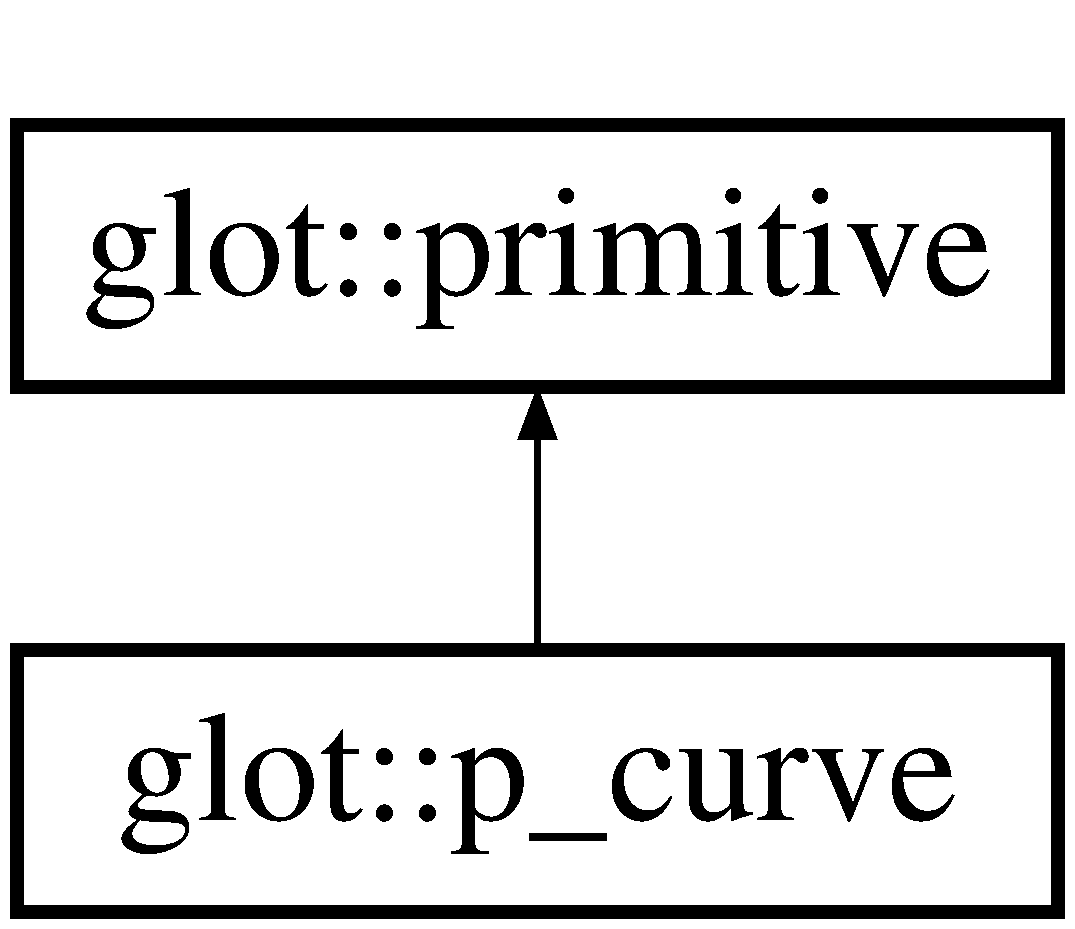
\includegraphics[height=2cm]{classglot_1_1p__curve}
\end{center}
\end{figure}
\subsection*{Public Member Functions}
\begin{CompactItemize}
\item 
{\bf p\_\-curve} (const {\bf function} \&x\_\-f, const {\bf function} \&y\_\-f, const {\bf color} \&col, double t0=0, double tf=1)
\begin{CompactList}\small\item\em Constructor. \item\end{CompactList}\item 
{\bf p\_\-curve} ({\bf function::double\_\-function} x\_\-f, {\bf function::double\_\-function} y\_\-f, const {\bf color} \&col, double t0=0, double tf=1)
\begin{CompactList}\small\item\em Constructor. \item\end{CompactList}\item 
double {\bf x} (double t)
\item 
double {\bf y} (double t)
\item 
void {\bf dl\_\-gen} (const {\bf screen} \&s)
\begin{CompactList}\small\item\em Display-list generator. \item\end{CompactList}\end{CompactItemize}
\subsection*{Public Attributes}
\begin{CompactItemize}
\item 
{\bf color} {\bf c}
\begin{CompactList}\small\item\em The \doxyref{color}{p.}{classglot_1_1color} of the the \doxyref{primitive}{p.}{classglot_1_1primitive}. \item\end{CompactList}\end{CompactItemize}
\subsection*{Protected Attributes}
\begin{CompactItemize}
\item 
{\bf function} {\bf x\_\-function}
\item 
{\bf function} {\bf y\_\-function}
\item 
double {\bf tstart}
\item 
double {\bf tfinal}
\end{CompactItemize}


\subsection{Detailed Description}
\doxyref{p\_\-curve}{p.}{classglot_1_1p__curve}: a parametric \doxyref{curve}{p.}{classglot_1_1curve} to plot 

This class takes two functions that accept doubles and return a double. It then samples t in [0,1] and connects the dots with straight lines

\begin{Desc}
\item[See also:]\doxyref{grapher}{p.}{classglot_1_1grapher} 

\doxyref{curve}{p.}{classglot_1_1curve} \end{Desc}


\subsection{Constructor \& Destructor Documentation}
\index{glot::p\_\-curve@{glot::p\_\-curve}!p\_\-curve@{p\_\-curve}}
\index{p\_\-curve@{p\_\-curve}!glot::p_curve@{glot::p\_\-curve}}
\subsubsection[{p\_\-curve}]{\setlength{\rightskip}{0pt plus 5cm}glot::p\_\-curve::p\_\-curve (const {\bf function} \& {\em x\_\-f}, \/  const {\bf function} \& {\em y\_\-f}, \/  const {\bf color} \& {\em col}, \/  double {\em t0} = {\tt 0}, \/  double {\em tf} = {\tt 1})\hspace{0.3cm}{\tt  [inline]}}\label{classglot_1_1p__curve_59b00998f11f0e4eb0102bd8255c0790}


Constructor. 

\begin{Desc}
\item[Parameters:]
\begin{description}
\item[{\em x\_\-f}]- the parametric definition of x \item[{\em y\_\-f}]- the parametric definition of y \item[{\em col}]- the \doxyref{color}{p.}{classglot_1_1color} of the \doxyref{curve}{p.}{classglot_1_1curve} \item[{\em t0}]- the beginning of the parameterization \item[{\em tf}]- the end of the parameterization \end{description}
\end{Desc}
\index{glot::p\_\-curve@{glot::p\_\-curve}!p\_\-curve@{p\_\-curve}}
\index{p\_\-curve@{p\_\-curve}!glot::p_curve@{glot::p\_\-curve}}
\subsubsection[{p\_\-curve}]{\setlength{\rightskip}{0pt plus 5cm}glot::p\_\-curve::p\_\-curve ({\bf function::double\_\-function} {\em x\_\-f}, \/  {\bf function::double\_\-function} {\em y\_\-f}, \/  const {\bf color} \& {\em col}, \/  double {\em t0} = {\tt 0}, \/  double {\em tf} = {\tt 1})\hspace{0.3cm}{\tt  [inline]}}\label{classglot_1_1p__curve_3f5facdd3e24ccd8fb27d60ffa7d913c}


Constructor. 

\begin{Desc}
\item[Parameters:]
\begin{description}
\item[{\em x\_\-f}]- the parametric definition of x \item[{\em y\_\-f}]- the parametric definition of y \item[{\em col}]- the \doxyref{color}{p.}{classglot_1_1color} of the \doxyref{curve}{p.}{classglot_1_1curve} \item[{\em t0}]- the beginning of the parameterization \item[{\em tf}]- the end of the parameterization\end{description}
\end{Desc}
Instead of declaring functions and a \doxyref{curve}{p.}{classglot_1_1curve}, we anticipate it being useful to just declare a \doxyref{curve}{p.}{classglot_1_1curve} with the functions you've already defined 

\subsection{Member Function Documentation}
\index{glot::p\_\-curve@{glot::p\_\-curve}!dl\_\-gen@{dl\_\-gen}}
\index{dl\_\-gen@{dl\_\-gen}!glot::p_curve@{glot::p\_\-curve}}
\subsubsection[{dl\_\-gen}]{\setlength{\rightskip}{0pt plus 5cm}void glot::p\_\-curve::dl\_\-gen (const {\bf screen} \& {\em s})\hspace{0.3cm}{\tt  [virtual]}}\label{classglot_1_1p__curve_2f746ce9f7acb0dc7b7ff5369219427e}


Display-list generator. 

\begin{Desc}
\item[Parameters:]
\begin{description}
\item[{\em s}]- the \doxyref{screen}{p.}{structscreen} specs\end{description}
\end{Desc}
The \doxyref{screen}{p.}{structscreen} stores the dimensions of the plot, etc. and based on that information, this \doxyref{function}{p.}{classglot_1_1function} generates the geometry for the \doxyref{primitive}{p.}{classglot_1_1primitive}. Typically this might be stored in a display list, but that is up to the container class, \doxyref{grapher}{p.}{classglot_1_1grapher} 

Implements {\bf glot::primitive} \doxyref{}{p.}{classglot_1_1primitive_2e8c612e7642561ae3536a865c08a436}.\index{glot::p\_\-curve@{glot::p\_\-curve}!x@{x}}
\index{x@{x}!glot::p_curve@{glot::p\_\-curve}}
\subsubsection[{x}]{\setlength{\rightskip}{0pt plus 5cm}double glot::p\_\-curve::x (double {\em t})}\label{classglot_1_1p__curve_b0a1092393f1ca36228bd2d4d58707f4}


\index{glot::p\_\-curve@{glot::p\_\-curve}!y@{y}}
\index{y@{y}!glot::p_curve@{glot::p\_\-curve}}
\subsubsection[{y}]{\setlength{\rightskip}{0pt plus 5cm}double glot::p\_\-curve::y (double {\em t})}\label{classglot_1_1p__curve_8b4d4c45556f00db419720bff1848e71}




\subsection{Member Data Documentation}
\index{glot::p\_\-curve@{glot::p\_\-curve}!c@{c}}
\index{c@{c}!glot::p_curve@{glot::p\_\-curve}}
\subsubsection[{c}]{\setlength{\rightskip}{0pt plus 5cm}{\bf color} {\bf glot::p\_\-curve::c}}\label{classglot_1_1p__curve_e322b3f013f9058bb063c1530e06e451}


The \doxyref{color}{p.}{classglot_1_1color} of the the \doxyref{primitive}{p.}{classglot_1_1primitive}. 



Reimplemented from {\bf glot::primitive} \doxyref{}{p.}{classglot_1_1primitive_ea0f7ab17148686a80fb68230eb09eba}.\index{glot::p\_\-curve@{glot::p\_\-curve}!tfinal@{tfinal}}
\index{tfinal@{tfinal}!glot::p_curve@{glot::p\_\-curve}}
\subsubsection[{tfinal}]{\setlength{\rightskip}{0pt plus 5cm}double {\bf glot::p\_\-curve::tfinal}\hspace{0.3cm}{\tt  [protected]}}\label{classglot_1_1p__curve_ab233c380c67f4b6e673d3476d08e9da}


\index{glot::p\_\-curve@{glot::p\_\-curve}!tstart@{tstart}}
\index{tstart@{tstart}!glot::p_curve@{glot::p\_\-curve}}
\subsubsection[{tstart}]{\setlength{\rightskip}{0pt plus 5cm}double {\bf glot::p\_\-curve::tstart}\hspace{0.3cm}{\tt  [protected]}}\label{classglot_1_1p__curve_ec011983027dcb5ac00c52e6c6b9f2f2}


\index{glot::p\_\-curve@{glot::p\_\-curve}!x\_\-function@{x\_\-function}}
\index{x\_\-function@{x\_\-function}!glot::p_curve@{glot::p\_\-curve}}
\subsubsection[{x\_\-function}]{\setlength{\rightskip}{0pt plus 5cm}{\bf function} {\bf glot::p\_\-curve::x\_\-function}\hspace{0.3cm}{\tt  [protected]}}\label{classglot_1_1p__curve_4f5bbaf2a346656ee808c6f3e00cb679}


\index{glot::p\_\-curve@{glot::p\_\-curve}!y\_\-function@{y\_\-function}}
\index{y\_\-function@{y\_\-function}!glot::p_curve@{glot::p\_\-curve}}
\subsubsection[{y\_\-function}]{\setlength{\rightskip}{0pt plus 5cm}{\bf function} {\bf glot::p\_\-curve::y\_\-function}\hspace{0.3cm}{\tt  [protected]}}\label{classglot_1_1p__curve_b1c4b399e8803f29bc2de9b52c3954ce}




The documentation for this class was generated from the following file:\begin{CompactItemize}
\item 
{\bf p\_\-curve.h}\end{CompactItemize}

\section{glot::point Class Reference}
\label{classglot_1_1point}\index{glot::point@{glot::point}}
{\tt \#include $<$point.h$>$}

\subsection*{Public Member Functions}
\begin{CompactItemize}
\item 
{\bf point} (double i, double j, double k, const {\bf color} \&col=NULL)
\begin{CompactList}\small\item\em Constructor. \item\end{CompactList}\end{CompactItemize}
\subsection*{Public Attributes}
\begin{CompactItemize}
\item 
{\bf color} {\bf c}
\begin{CompactList}\small\item\em The \doxyref{color}{p.}{classglot_1_1color} of the the \doxyref{point}{p.}{classglot_1_1point}. \item\end{CompactList}\item 
double {\bf x}
\begin{CompactList}\small\item\em The x coordinate of the \doxyref{point}{p.}{classglot_1_1point}. \item\end{CompactList}\item 
double {\bf y}
\begin{CompactList}\small\item\em The y coordinate of the \doxyref{point}{p.}{classglot_1_1point}. \item\end{CompactList}\item 
double {\bf z}
\begin{CompactList}\small\item\em The z coordinate of the \doxyref{point}{p.}{classglot_1_1point}. \item\end{CompactList}\end{CompactItemize}


\subsection{Constructor \& Destructor Documentation}
\index{glot::point@{glot::point}!point@{point}}
\index{point@{point}!glot::point@{glot::point}}
\subsubsection[{point}]{\setlength{\rightskip}{0pt plus 5cm}glot::point::point (double {\em i}, \/  double {\em j}, \/  double {\em k}, \/  const {\bf color} \& {\em col} = {\tt NULL})\hspace{0.3cm}{\tt  [inline]}}\label{classglot_1_1point_f6a211d8f56ac6a64fe7c4e136410af2}


Constructor. 

\begin{Desc}
\item[Parameters:]
\begin{description}
\item[{\em i}]- the x coordinate of the \doxyref{point}{p.}{classglot_1_1point} \item[{\em j}]- the y coordinate of the \doxyref{point}{p.}{classglot_1_1point} \item[{\em k}]- the z coordinate of the \doxyref{point}{p.}{classglot_1_1point} \item[{\em col}]- the \doxyref{color}{p.}{classglot_1_1color} with which to draw \end{description}
\end{Desc}


\subsection{Member Data Documentation}
\index{glot::point@{glot::point}!c@{c}}
\index{c@{c}!glot::point@{glot::point}}
\subsubsection[{c}]{\setlength{\rightskip}{0pt plus 5cm}{\bf color} {\bf glot::point::c}}\label{classglot_1_1point_cbddc5e3b7988c242759b60e07d50a8a}


The \doxyref{color}{p.}{classglot_1_1color} of the the \doxyref{point}{p.}{classglot_1_1point}. 

\index{glot::point@{glot::point}!x@{x}}
\index{x@{x}!glot::point@{glot::point}}
\subsubsection[{x}]{\setlength{\rightskip}{0pt plus 5cm}double {\bf glot::point::x}}\label{classglot_1_1point_eb96e64adf81606e8cb0a32506165fa9}


The x coordinate of the \doxyref{point}{p.}{classglot_1_1point}. 

\index{glot::point@{glot::point}!y@{y}}
\index{y@{y}!glot::point@{glot::point}}
\subsubsection[{y}]{\setlength{\rightskip}{0pt plus 5cm}double {\bf glot::point::y}}\label{classglot_1_1point_93fb999d115305f6571f213528203be9}


The y coordinate of the \doxyref{point}{p.}{classglot_1_1point}. 

\index{glot::point@{glot::point}!z@{z}}
\index{z@{z}!glot::point@{glot::point}}
\subsubsection[{z}]{\setlength{\rightskip}{0pt plus 5cm}double {\bf glot::point::z}}\label{classglot_1_1point_0f2aa2d9c3b19dfe40f0f424e9626fb6}


The z coordinate of the \doxyref{point}{p.}{classglot_1_1point}. 



The documentation for this class was generated from the following file:\begin{CompactItemize}
\item 
{\bf point.h}\end{CompactItemize}

\section{glot::primitive Class Reference}
\label{classglot_1_1primitive}\index{glot::primitive@{glot::primitive}}
\doxyref{primitive}{p.}{classglot_1_1primitive}: the parent class of all rendered objects  


{\tt \#include $<$primitive.h$>$}

Inheritance diagram for glot::primitive::\begin{figure}[H]
\begin{center}
\leavevmode
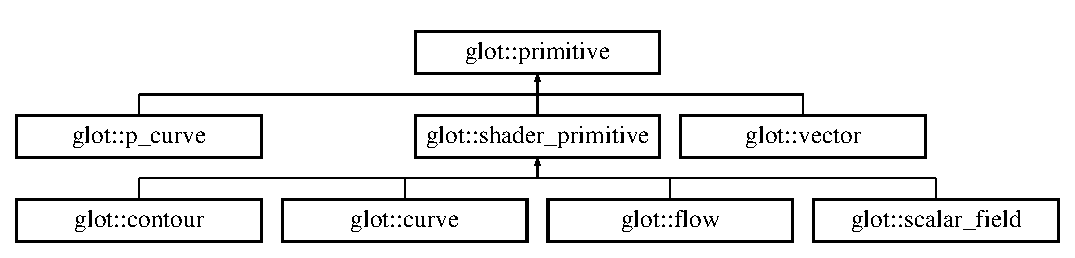
\includegraphics[height=3cm]{classglot_1_1primitive}
\end{center}
\end{figure}
\subsection*{Public Member Functions}
\begin{CompactItemize}
\item 
{\bf primitive} ()
\begin{CompactList}\small\item\em Default constructor. \item\end{CompactList}\item 
{\bf primitive} (const {\bf color} \&col)
\begin{CompactList}\small\item\em Constructor. \item\end{CompactList}\item 
virtual {\bf $\sim$primitive} ()
\begin{CompactList}\small\item\em Destructor. \item\end{CompactList}\item 
virtual void {\bf dl\_\-gen} (const {\bf screen} \&s)=0
\begin{CompactList}\small\item\em Display-list generator. \item\end{CompactList}\end{CompactItemize}
\subsection*{Public Attributes}
\begin{CompactItemize}
\item 
{\bf color} {\bf c}
\begin{CompactList}\small\item\em The \doxyref{color}{p.}{classglot_1_1color} of the the \doxyref{primitive}{p.}{classglot_1_1primitive}. \item\end{CompactList}\item 
GLenum {\bf p}
\begin{CompactList}\small\item\em Shader program handle. \item\end{CompactList}\end{CompactItemize}


\subsection{Detailed Description}
\doxyref{primitive}{p.}{classglot_1_1primitive}: the parent class of all rendered objects 

This class is the parent of all the primitives that get drawn to the \doxyref{screen}{p.}{structscreen}.

\begin{Desc}
\item[See also:]\doxyref{shader\_\-primitive}{p.}{classglot_1_1shader__primitive} \end{Desc}


\subsection{Constructor \& Destructor Documentation}
\index{glot::primitive@{glot::primitive}!primitive@{primitive}}
\index{primitive@{primitive}!glot::primitive@{glot::primitive}}
\subsubsection[{primitive}]{\setlength{\rightskip}{0pt plus 5cm}glot::primitive::primitive ()\hspace{0.3cm}{\tt  [inline]}}\label{classglot_1_1primitive_db78c0195a775307e565a696d4daaa99}


Default constructor. 

\index{glot::primitive@{glot::primitive}!primitive@{primitive}}
\index{primitive@{primitive}!glot::primitive@{glot::primitive}}
\subsubsection[{primitive}]{\setlength{\rightskip}{0pt plus 5cm}glot::primitive::primitive (const {\bf color} \& {\em col})\hspace{0.3cm}{\tt  [inline]}}\label{classglot_1_1primitive_0e1f934674a70902f0221d7319f18186}


Constructor. 

\begin{Desc}
\item[Parameters:]
\begin{description}
\item[{\em col}]- the \doxyref{color}{p.}{classglot_1_1color} of the \doxyref{primitive}{p.}{classglot_1_1primitive}\end{description}
\end{Desc}
Initializes the \doxyref{color}{p.}{classglot_1_1color} of the \doxyref{primitive}{p.}{classglot_1_1primitive} and the program GLenum \index{glot::primitive@{glot::primitive}!$\sim$primitive@{$\sim$primitive}}
\index{$\sim$primitive@{$\sim$primitive}!glot::primitive@{glot::primitive}}
\subsubsection[{$\sim$primitive}]{\setlength{\rightskip}{0pt plus 5cm}virtual glot::primitive::$\sim$primitive ()\hspace{0.3cm}{\tt  [inline, virtual]}}\label{classglot_1_1primitive_7c5a2b51466cde951ac85b6c86309cca}


Destructor. 

Virtual classes need virtual destructors 

\subsection{Member Function Documentation}
\index{glot::primitive@{glot::primitive}!dl\_\-gen@{dl\_\-gen}}
\index{dl\_\-gen@{dl\_\-gen}!glot::primitive@{glot::primitive}}
\subsubsection[{dl\_\-gen}]{\setlength{\rightskip}{0pt plus 5cm}virtual void glot::primitive::dl\_\-gen (const {\bf screen} \& {\em s})\hspace{0.3cm}{\tt  [pure virtual]}}\label{classglot_1_1primitive_2e8c612e7642561ae3536a865c08a436}


Display-list generator. 

\begin{Desc}
\item[Parameters:]
\begin{description}
\item[{\em s}]- the \doxyref{screen}{p.}{structscreen} specs\end{description}
\end{Desc}
The \doxyref{screen}{p.}{structscreen} stores the dimensions of the plot, etc. and based on that information, this \doxyref{function}{p.}{classglot_1_1function} generates the geometry for the \doxyref{primitive}{p.}{classglot_1_1primitive}. Typically this might be stored in a display list, but that is up to the container class, \doxyref{grapher}{p.}{classglot_1_1grapher} 

Implemented in {\bf glot::contour} \doxyref{}{p.}{classglot_1_1contour_ad1f9a15676372dfb398e68772f59625}, {\bf glot::curve} \doxyref{}{p.}{classglot_1_1curve_29cf8bdce745306212af7c147023fba4}, {\bf glot::flow} \doxyref{}{p.}{classglot_1_1flow_9b7fb4fd93ca8b9938b65e5810e4b596}, {\bf glot::p\_\-curve} \doxyref{}{p.}{classglot_1_1p__curve_2f746ce9f7acb0dc7b7ff5369219427e}, {\bf glot::scalar\_\-field} \doxyref{}{p.}{classglot_1_1scalar__field_269705f742e38107a915147d45fdb569}, and {\bf glot::vector} \doxyref{}{p.}{classglot_1_1vector_ba40ac7886d92d63fc9d7f198643929d}.

\subsection{Member Data Documentation}
\index{glot::primitive@{glot::primitive}!c@{c}}
\index{c@{c}!glot::primitive@{glot::primitive}}
\subsubsection[{c}]{\setlength{\rightskip}{0pt plus 5cm}{\bf color} {\bf glot::primitive::c}}\label{classglot_1_1primitive_ea0f7ab17148686a80fb68230eb09eba}


The \doxyref{color}{p.}{classglot_1_1color} of the the \doxyref{primitive}{p.}{classglot_1_1primitive}. 



Reimplemented in {\bf glot::curve} \doxyref{}{p.}{classglot_1_1curve_fcd83ec8bb2dbcb8b148a192f0a9c99b}, {\bf glot::p\_\-curve} \doxyref{}{p.}{classglot_1_1p__curve_e322b3f013f9058bb063c1530e06e451}, and {\bf glot::vector} \doxyref{}{p.}{classglot_1_1vector_97ca7ee8b946ffe4b9950b6255663168}.\index{glot::primitive@{glot::primitive}!p@{p}}
\index{p@{p}!glot::primitive@{glot::primitive}}
\subsubsection[{p}]{\setlength{\rightskip}{0pt plus 5cm}GLenum {\bf glot::primitive::p}}\label{classglot_1_1primitive_e0c4cfa6abb55f0a13c6e12fac732f9b}


Shader program handle. 

Some primitives specify their own shader programs and the container class, \doxyref{grapher}{p.}{classglot_1_1grapher}, will use each one's self-specified program when it's called. 

The documentation for this class was generated from the following file:\begin{CompactItemize}
\item 
{\bf primitive.h}\end{CompactItemize}

\section{glot::scalar\_\-field Class Reference}
\label{classglot_1_1scalar__field}\index{glot::scalar\_\-field@{glot::scalar\_\-field}}
\doxyref{scalar\_\-field}{p.}{classglot_1_1scalar__field}: a scalar field to plot  


{\tt \#include $<$scalar\_\-field.h$>$}

Inheritance diagram for glot::scalar\_\-field::\begin{figure}[H]
\begin{center}
\leavevmode
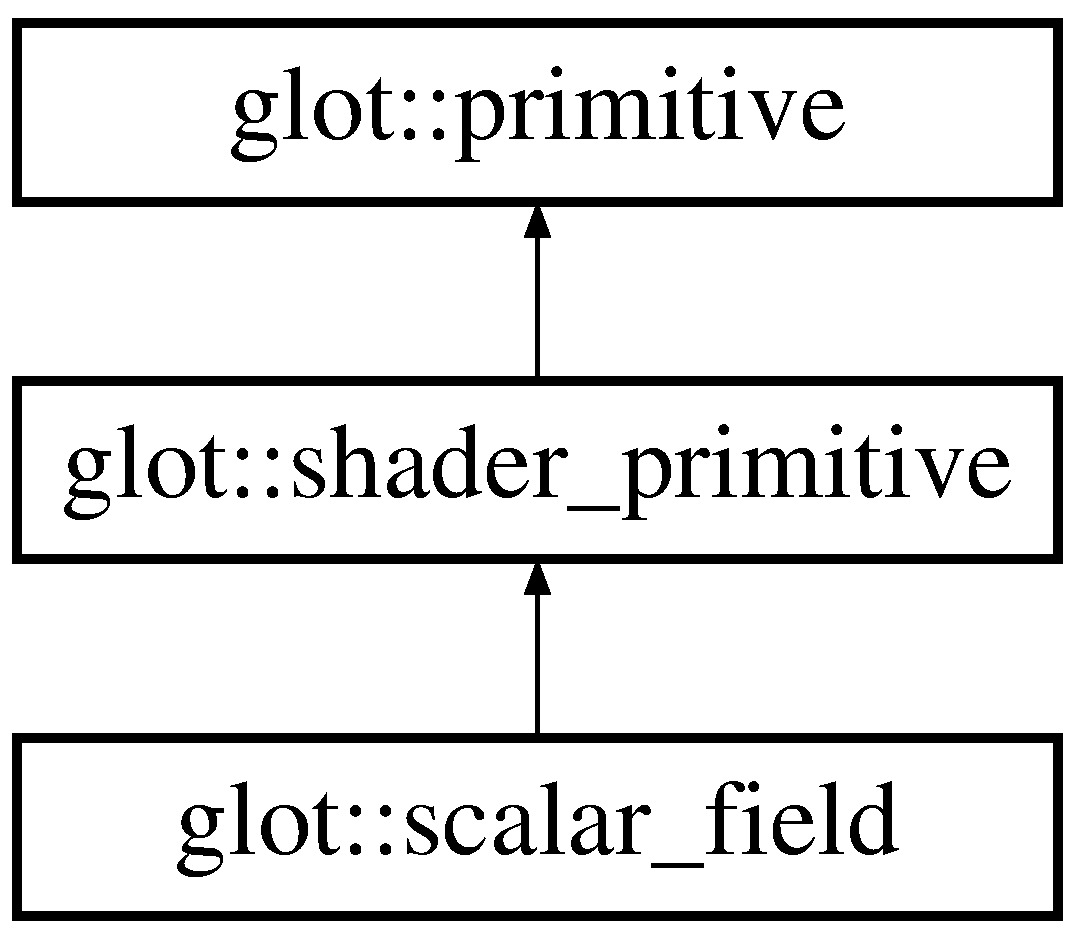
\includegraphics[height=3cm]{classglot_1_1scalar__field}
\end{center}
\end{figure}
\subsection*{Public Member Functions}
\begin{CompactItemize}
\item 
{\bf scalar\_\-field} (const string \&{\bf f})
\begin{CompactList}\small\item\em Constructor. \item\end{CompactList}\item 
void {\bf dl\_\-gen} (const {\bf screen} \&s)
\begin{CompactList}\small\item\em Display-list generator. \item\end{CompactList}\end{CompactItemize}


\subsection{Detailed Description}
\doxyref{scalar\_\-field}{p.}{classglot_1_1scalar__field}: a scalar field to plot 

This class takes a scalar-valued \doxyref{function}{p.}{classglot_1_1function} of x, y and t and renders the resulting scalar field with a fragment shader. The shader expects the value of the \doxyref{function}{p.}{classglot_1_1function} to be scaled between -1 and 1 and will clamp any value outside of that. (For instance, -10 gets mapped to the \doxyref{color}{p.}{classglot_1_1color} for -1 and 1220 gets mapped to the value for 1).

Future versions will allow for a user-specified range, and ideally would also have a mode that automatically scales the values appropriately.

\begin{Desc}
\item[See also:]\doxyref{grapher}{p.}{classglot_1_1grapher} 

\doxyref{p\_\-curve}{p.}{classglot_1_1p__curve} \end{Desc}


\subsection{Constructor \& Destructor Documentation}
\index{glot::scalar\_\-field@{glot::scalar\_\-field}!scalar\_\-field@{scalar\_\-field}}
\index{scalar\_\-field@{scalar\_\-field}!glot::scalar_field@{glot::scalar\_\-field}}
\subsubsection[{scalar\_\-field}]{\setlength{\rightskip}{0pt plus 5cm}glot::scalar\_\-field::scalar\_\-field (const string \& {\em f})\hspace{0.3cm}{\tt  [inline]}}\label{classglot_1_1scalar__field_d475702f28186bdc406ffc70eaa7a04a}


Constructor. 

\begin{Desc}
\item[Parameters:]
\begin{description}
\item[{\em func}]- the \doxyref{function}{p.}{classglot_1_1function} to render \end{description}
\end{Desc}


\subsection{Member Function Documentation}
\index{glot::scalar\_\-field@{glot::scalar\_\-field}!dl\_\-gen@{dl\_\-gen}}
\index{dl\_\-gen@{dl\_\-gen}!glot::scalar_field@{glot::scalar\_\-field}}
\subsubsection[{dl\_\-gen}]{\setlength{\rightskip}{0pt plus 5cm}void glot::scalar\_\-field::dl\_\-gen (const {\bf screen} \& {\em s})\hspace{0.3cm}{\tt  [virtual]}}\label{classglot_1_1scalar__field_269705f742e38107a915147d45fdb569}


Display-list generator. 

\begin{Desc}
\item[Parameters:]
\begin{description}
\item[{\em s}]- the \doxyref{screen}{p.}{structscreen} specs of the plot\end{description}
\end{Desc}
Generates a screen-filling quad that serves as the canvas for the fragment shader to do its thing. 

Implements {\bf glot::primitive} \doxyref{}{p.}{classglot_1_1primitive_2e8c612e7642561ae3536a865c08a436}.

The documentation for this class was generated from the following file:\begin{CompactItemize}
\item 
{\bf scalar\_\-field.h}\end{CompactItemize}

\section{screen Struct Reference}
\label{structscreen}\index{screen@{screen}}
{\tt \#include $<$screen.h$>$}

\subsection*{Public Attributes}
\begin{CompactItemize}
\item 
int {\bf height}
\item 
int {\bf width}
\item 
double {\bf minx}
\item 
double {\bf maxx}
\item 
double {\bf miny}
\item 
double {\bf maxy}
\item 
double {\bf time}
\end{CompactItemize}


\subsection{Member Data Documentation}
\index{screen@{screen}!height@{height}}
\index{height@{height}!screen@{screen}}
\subsubsection[{height}]{\setlength{\rightskip}{0pt plus 5cm}int {\bf screen::height}}\label{structscreen_bf92d5370ef230dd4c6f603435341f50}


\index{screen@{screen}!maxx@{maxx}}
\index{maxx@{maxx}!screen@{screen}}
\subsubsection[{maxx}]{\setlength{\rightskip}{0pt plus 5cm}double {\bf screen::maxx}}\label{structscreen_44a54fff987e77df78e735135c49a06c}


\index{screen@{screen}!maxy@{maxy}}
\index{maxy@{maxy}!screen@{screen}}
\subsubsection[{maxy}]{\setlength{\rightskip}{0pt plus 5cm}double {\bf screen::maxy}}\label{structscreen_ed903ce1e7c63258fff721dd7589d664}


\index{screen@{screen}!minx@{minx}}
\index{minx@{minx}!screen@{screen}}
\subsubsection[{minx}]{\setlength{\rightskip}{0pt plus 5cm}double {\bf screen::minx}}\label{structscreen_ce1577a6c8685aa8aabb3008346ee014}


\index{screen@{screen}!miny@{miny}}
\index{miny@{miny}!screen@{screen}}
\subsubsection[{miny}]{\setlength{\rightskip}{0pt plus 5cm}double {\bf screen::miny}}\label{structscreen_e58c495356145ced9399aa6fe2fe36e4}


\index{screen@{screen}!time@{time}}
\index{time@{time}!screen@{screen}}
\subsubsection[{time}]{\setlength{\rightskip}{0pt plus 5cm}double {\bf screen::time}}\label{structscreen_823fed6a66633783f3d828ac2fdf21dd}


\index{screen@{screen}!width@{width}}
\index{width@{width}!screen@{screen}}
\subsubsection[{width}]{\setlength{\rightskip}{0pt plus 5cm}int {\bf screen::width}}\label{structscreen_5a1821f8d8c202dfbf0755d2162fb64b}




The documentation for this struct was generated from the following file:\begin{CompactItemize}
\item 
{\bf screen.h}\end{CompactItemize}

\section{glot::shader\_\-primitive Class Reference}
\label{classglot_1_1shader__primitive}\index{glot::shader\_\-primitive@{glot::shader\_\-primitive}}
\doxyref{shader\_\-primitive}{p.}{classglot_1_1shader__primitive}: the parent class of all primitives that use their own shaders  


{\tt \#include $<$shader\_\-primitive.h$>$}

Inheritance diagram for glot::shader\_\-primitive::\begin{figure}[H]
\begin{center}
\leavevmode
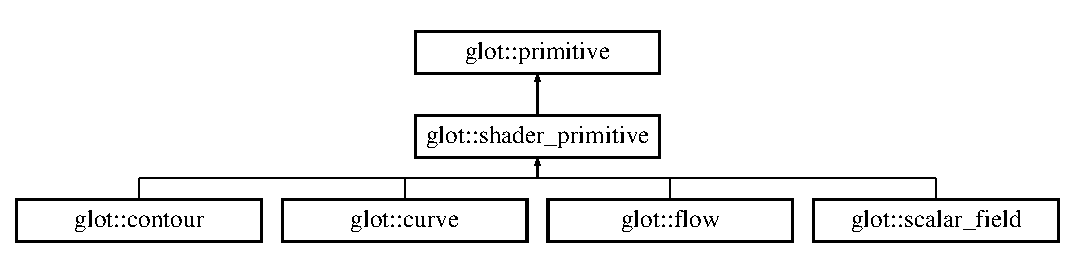
\includegraphics[height=3cm]{classglot_1_1shader__primitive}
\end{center}
\end{figure}
\subsection*{Public Member Functions}
\begin{CompactItemize}
\item 
{\bf shader\_\-primitive} ()
\begin{CompactList}\small\item\em Default constructor. \item\end{CompactList}\item 
{\bf shader\_\-primitive} (const {\bf color} \&col)
\begin{CompactList}\small\item\em Constructor. \item\end{CompactList}\item 
virtual {\bf $\sim$shader\_\-primitive} ()
\begin{CompactList}\small\item\em Destructor. \item\end{CompactList}\item 
void {\bf printProgramInfoLog} (GLuint obj)
\begin{CompactList}\small\item\em Program linking errors. \item\end{CompactList}\item 
void {\bf printShaderInfoLog} (GLuint obj)
\begin{CompactList}\small\item\em Shader compiling errors. \item\end{CompactList}\item 
string {\bf read\_\-file} (const char $\ast$filename)
\begin{CompactList}\small\item\em Read in a file. \item\end{CompactList}\end{CompactItemize}
\subsection*{Protected Attributes}
\begin{CompactItemize}
\item 
GLhandleARB {\bf f}
\begin{CompactList}\small\item\em Shader source handles. \item\end{CompactList}\item 
GLhandleARB {\bf g}
\item 
GLhandleARB {\bf v}
\end{CompactItemize}


\subsection{Detailed Description}
\doxyref{shader\_\-primitive}{p.}{classglot_1_1shader__primitive}: the parent class of all primitives that use their own shaders 

This class is the parent of all the primitives that get drawn to the \doxyref{screen}{p.}{structscreen} but use their own shaders. It helps out by providing a few helpful functions for compiling shader programs and reading files and so forth.

\begin{Desc}
\item[See also:]\doxyref{shader\_\-primitive}{p.}{classglot_1_1shader__primitive} \end{Desc}


\subsection{Constructor \& Destructor Documentation}
\index{glot::shader\_\-primitive@{glot::shader\_\-primitive}!shader\_\-primitive@{shader\_\-primitive}}
\index{shader\_\-primitive@{shader\_\-primitive}!glot::shader_primitive@{glot::shader\_\-primitive}}
\subsubsection[{shader\_\-primitive}]{\setlength{\rightskip}{0pt plus 5cm}glot::shader\_\-primitive::shader\_\-primitive ()\hspace{0.3cm}{\tt  [inline]}}\label{classglot_1_1shader__primitive_2bacef1be37a4a4805bdbfa8c7679db2}


Default constructor. 

\index{glot::shader\_\-primitive@{glot::shader\_\-primitive}!shader\_\-primitive@{shader\_\-primitive}}
\index{shader\_\-primitive@{shader\_\-primitive}!glot::shader_primitive@{glot::shader\_\-primitive}}
\subsubsection[{shader\_\-primitive}]{\setlength{\rightskip}{0pt plus 5cm}glot::shader\_\-primitive::shader\_\-primitive (const {\bf color} \& {\em col})\hspace{0.3cm}{\tt  [inline]}}\label{classglot_1_1shader__primitive_1b24678b292e10204f97c7c8c2732a23}


Constructor. 

\begin{Desc}
\item[Parameters:]
\begin{description}
\item[{\em col}]- the \doxyref{color}{p.}{classglot_1_1color} of the \doxyref{primitive}{p.}{classglot_1_1primitive} \end{description}
\end{Desc}
\index{glot::shader\_\-primitive@{glot::shader\_\-primitive}!$\sim$shader\_\-primitive@{$\sim$shader\_\-primitive}}
\index{$\sim$shader\_\-primitive@{$\sim$shader\_\-primitive}!glot::shader_primitive@{glot::shader\_\-primitive}}
\subsubsection[{$\sim$shader\_\-primitive}]{\setlength{\rightskip}{0pt plus 5cm}virtual glot::shader\_\-primitive::$\sim$shader\_\-primitive ()\hspace{0.3cm}{\tt  [inline, virtual]}}\label{classglot_1_1shader__primitive_93bfea81ab50ae43ce5c8812654271f0}


Destructor. 

Virtual classes need virtual destructors 

\subsection{Member Function Documentation}
\index{glot::shader\_\-primitive@{glot::shader\_\-primitive}!printProgramInfoLog@{printProgramInfoLog}}
\index{printProgramInfoLog@{printProgramInfoLog}!glot::shader_primitive@{glot::shader\_\-primitive}}
\subsubsection[{printProgramInfoLog}]{\setlength{\rightskip}{0pt plus 5cm}void glot::shader\_\-primitive::printProgramInfoLog (GLuint {\em obj})}\label{classglot_1_1shader__primitive_1f240d0f05e89e381c35450390128061}


Program linking errors. 

\begin{Desc}
\item[Parameters:]
\begin{description}
\item[{\em obj}]- the program to talk about\end{description}
\end{Desc}
This \doxyref{function}{p.}{classglot_1_1function} prints out information about the linking stage of the GLSL shader program generation. GLSL prefers to fail silently, but provides ways to query back on the status of the linking of the shader program and this provides a way to check on that status in a human-readable format.

I found this helpful \doxyref{function}{p.}{classglot_1_1function} at: {\tt http://www.lighthouse3d.com/opengl/glsl/index.php?oglinfo} \index{glot::shader\_\-primitive@{glot::shader\_\-primitive}!printShaderInfoLog@{printShaderInfoLog}}
\index{printShaderInfoLog@{printShaderInfoLog}!glot::shader_primitive@{glot::shader\_\-primitive}}
\subsubsection[{printShaderInfoLog}]{\setlength{\rightskip}{0pt plus 5cm}void glot::shader\_\-primitive::printShaderInfoLog (GLuint {\em obj})}\label{classglot_1_1shader__primitive_8ebd19ffbde159147225a276448e35f1}


Shader compiling errors. 

\begin{Desc}
\item[Parameters:]
\begin{description}
\item[{\em obj}]- the shader to talk about\end{description}
\end{Desc}
This \doxyref{function}{p.}{classglot_1_1function} prints out information about the compiling of the GLSL shader. GLSL fails silently, but has a way to the status of the compilation of a shader and this prints out that information.

I found this helpful \doxyref{function}{p.}{classglot_1_1function} at: {\tt http://www.lighthouse3d.com/opengl/glsl/index.php?oglinfo} \index{glot::shader\_\-primitive@{glot::shader\_\-primitive}!read\_\-file@{read\_\-file}}
\index{read\_\-file@{read\_\-file}!glot::shader_primitive@{glot::shader\_\-primitive}}
\subsubsection[{read\_\-file}]{\setlength{\rightskip}{0pt plus 5cm}string glot::shader\_\-primitive::read\_\-file (const char $\ast$ {\em filename})}\label{classglot_1_1shader__primitive_a56ca0b59dd09e40d37670ef74ff1bb9}


Read in a file. 

\begin{Desc}
\item[Parameters:]
\begin{description}
\item[{\em filename}]- the name of the file to read\end{description}
\end{Desc}
Reads a file, returns a string with the contents of that file. Meant to facilitate reading in the shader source, which is usually stored in a file. 

\subsection{Member Data Documentation}
\index{glot::shader\_\-primitive@{glot::shader\_\-primitive}!f@{f}}
\index{f@{f}!glot::shader_primitive@{glot::shader\_\-primitive}}
\subsubsection[{f}]{\setlength{\rightskip}{0pt plus 5cm}GLhandleARB {\bf glot::shader\_\-primitive::f}\hspace{0.3cm}{\tt  [protected]}}\label{classglot_1_1shader__primitive_36d2a7a1bc7302406c7f0af5b23ed9c9}


Shader source handles. 

I'm not entirely sure if it's necessary to store these handles beyond the compiling and then linking the shader program, but these are for that purpose. \index{glot::shader\_\-primitive@{glot::shader\_\-primitive}!g@{g}}
\index{g@{g}!glot::shader_primitive@{glot::shader\_\-primitive}}
\subsubsection[{g}]{\setlength{\rightskip}{0pt plus 5cm}GLhandleARB {\bf glot::shader\_\-primitive::g}\hspace{0.3cm}{\tt  [protected]}}\label{classglot_1_1shader__primitive_0681d4187ae1a8cbc8cc729dc48c7b5a}


\index{glot::shader\_\-primitive@{glot::shader\_\-primitive}!v@{v}}
\index{v@{v}!glot::shader_primitive@{glot::shader\_\-primitive}}
\subsubsection[{v}]{\setlength{\rightskip}{0pt plus 5cm}GLhandleARB {\bf glot::shader\_\-primitive::v}\hspace{0.3cm}{\tt  [protected]}}\label{classglot_1_1shader__primitive_002e1317b915ca6339f2a8b826823b63}




The documentation for this class was generated from the following file:\begin{CompactItemize}
\item 
{\bf shader\_\-primitive.h}\end{CompactItemize}

\section{stopwatch Class Reference}
\label{classstopwatch}\index{stopwatch@{stopwatch}}
\doxyref{stopwatch}{p.}{classstopwatch} : encapsulates timing routines  


{\tt \#include $<$stopwatch.h$>$}

\subsection*{Public Member Functions}
\begin{CompactItemize}
\item 
{\bf stopwatch} ()
\begin{CompactList}\small\item\em Constructor. \item\end{CompactList}\item 
void {\bf start} ()
\begin{CompactList}\small\item\em Start the \doxyref{stopwatch}{p.}{classstopwatch}. \item\end{CompactList}\item 
double {\bf time} ()
\begin{CompactList}\small\item\em Get the current time of the \doxyref{stopwatch}{p.}{classstopwatch}. \item\end{CompactList}\item 
double {\bf stop} ()
\begin{CompactList}\small\item\em Stop the \doxyref{stopwatch}{p.}{classstopwatch}, get the time. \item\end{CompactList}\end{CompactItemize}


\subsection{Detailed Description}
\doxyref{stopwatch}{p.}{classstopwatch} : encapsulates timing routines 

This class encapsulates the system's timing functions. I've found that Mac and Linux use very different versions of time.h, and with different clock resolutions. Rather than deal with it in the silly C-style (this is C++ after all), I created a simple \doxyref{stopwatch}{p.}{classstopwatch} class. 

\subsection{Constructor \& Destructor Documentation}
\index{stopwatch@{stopwatch}!stopwatch@{stopwatch}}
\index{stopwatch@{stopwatch}!stopwatch@{stopwatch}}
\subsubsection[{stopwatch}]{\setlength{\rightskip}{0pt plus 5cm}stopwatch::stopwatch ()\hspace{0.3cm}{\tt  [inline]}}\label{classstopwatch_427b7eff0db59c70a0239dc354b4323e}


Constructor. 



\subsection{Member Function Documentation}
\index{stopwatch@{stopwatch}!start@{start}}
\index{start@{start}!stopwatch@{stopwatch}}
\subsubsection[{start}]{\setlength{\rightskip}{0pt plus 5cm}void stopwatch::start ()}\label{classstopwatch_875bf8a472dff32a8190ec96e7fcf969}


Start the \doxyref{stopwatch}{p.}{classstopwatch}. 

Start the timing of the \doxyref{stopwatch}{p.}{classstopwatch}, just records the current WALL TIME. This does not measure anything but the wall time. Not system time, not clock cycles just the wall time. \index{stopwatch@{stopwatch}!stop@{stop}}
\index{stop@{stop}!stopwatch@{stopwatch}}
\subsubsection[{stop}]{\setlength{\rightskip}{0pt plus 5cm}double stopwatch::stop ()}\label{classstopwatch_3bfa7f394f995ffa8ef866d1391e97cd}


Stop the \doxyref{stopwatch}{p.}{classstopwatch}, get the time. 

This returns the stopwatch's current time and does stop it. Returns the time in seconds as a double \index{stopwatch@{stopwatch}!time@{time}}
\index{time@{time}!stopwatch@{stopwatch}}
\subsubsection[{time}]{\setlength{\rightskip}{0pt plus 5cm}double stopwatch::time ()}\label{classstopwatch_4d224136091cc2e66e078ddd09ea4c73}


Get the current time of the \doxyref{stopwatch}{p.}{classstopwatch}. 

This returns the stopwatch's current time without stopping it. Returns the time in seconds as a double 

The documentation for this class was generated from the following file:\begin{CompactItemize}
\item 
{\bf stopwatch.h}\end{CompactItemize}

\section{glot::vector Class Reference}
\label{classglot_1_1vector}\index{glot::vector@{glot::vector}}
{\tt \#include $<$vector.h$>$}

Inheritance diagram for glot::vector::\begin{figure}[H]
\begin{center}
\leavevmode
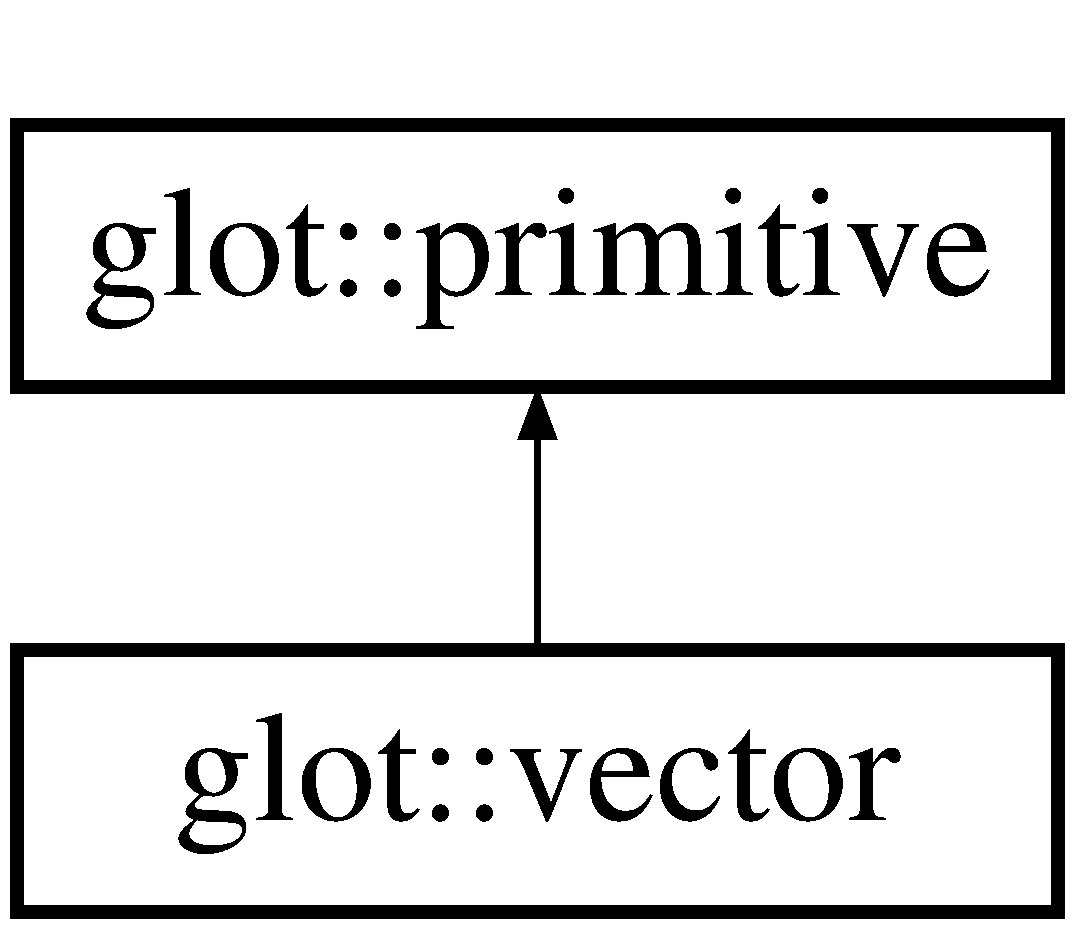
\includegraphics[height=2cm]{classglot_1_1vector}
\end{center}
\end{figure}
\subsection*{Public Member Functions}
\begin{CompactItemize}
\item 
{\bf vector} (const {\bf point} \&s, const {\bf point} \&e, const {\bf color} \&col)
\begin{CompactList}\small\item\em Constructor. \item\end{CompactList}\item 
void {\bf dl\_\-gen} (const {\bf screen} \&s)
\begin{CompactList}\small\item\em Display-list generator. \item\end{CompactList}\end{CompactItemize}
\subsection*{Public Attributes}
\begin{CompactItemize}
\item 
{\bf color} {\bf c}
\begin{CompactList}\small\item\em The \doxyref{color}{p.}{classglot_1_1color} of the the \doxyref{point}{p.}{classglot_1_1point}. \item\end{CompactList}\item 
{\bf point} {\bf start}
\begin{CompactList}\small\item\em The endpoints of the \doxyref{vector}{p.}{classglot_1_1vector}. \item\end{CompactList}\item 
{\bf point} {\bf end}
\end{CompactItemize}


\subsection{Constructor \& Destructor Documentation}
\index{glot::vector@{glot::vector}!vector@{vector}}
\index{vector@{vector}!glot::vector@{glot::vector}}
\subsubsection[{vector}]{\setlength{\rightskip}{0pt plus 5cm}glot::vector::vector (const {\bf point} \& {\em s}, \/  const {\bf point} \& {\em e}, \/  const {\bf color} \& {\em col})\hspace{0.3cm}{\tt  [inline]}}\label{classglot_1_1vector_e0764b96dea37eae5b0c69b7a651ef44}


Constructor. 

\begin{Desc}
\item[Parameters:]
\begin{description}
\item[{\em s}]- the start \doxyref{point}{p.}{classglot_1_1point} \item[{\em e}]- the end \doxyref{point}{p.}{classglot_1_1point} \item[{\em col}]- the \doxyref{color}{p.}{classglot_1_1color} with which to draw \end{description}
\end{Desc}


\subsection{Member Function Documentation}
\index{glot::vector@{glot::vector}!dl\_\-gen@{dl\_\-gen}}
\index{dl\_\-gen@{dl\_\-gen}!glot::vector@{glot::vector}}
\subsubsection[{dl\_\-gen}]{\setlength{\rightskip}{0pt plus 5cm}void glot::vector::dl\_\-gen (const {\bf screen} \& {\em s})\hspace{0.3cm}{\tt  [virtual]}}\label{classglot_1_1vector_ba40ac7886d92d63fc9d7f198643929d}


Display-list generator. 

\begin{Desc}
\item[Parameters:]
\begin{description}
\item[{\em s}]- the \doxyref{screen}{p.}{structscreen} specs\end{description}
\end{Desc}
The \doxyref{screen}{p.}{structscreen} stores the dimensions of the plot, etc. and based on that information, this \doxyref{function}{p.}{classglot_1_1function} generates the geometry for the \doxyref{primitive}{p.}{classglot_1_1primitive}. Typically this might be stored in a display list, but that is up to the container class, \doxyref{grapher}{p.}{classglot_1_1grapher} 

Implements {\bf glot::primitive} \doxyref{}{p.}{classglot_1_1primitive_2e8c612e7642561ae3536a865c08a436}.

\subsection{Member Data Documentation}
\index{glot::vector@{glot::vector}!c@{c}}
\index{c@{c}!glot::vector@{glot::vector}}
\subsubsection[{c}]{\setlength{\rightskip}{0pt plus 5cm}{\bf color} {\bf glot::vector::c}}\label{classglot_1_1vector_97ca7ee8b946ffe4b9950b6255663168}


The \doxyref{color}{p.}{classglot_1_1color} of the the \doxyref{point}{p.}{classglot_1_1point}. 



Reimplemented from {\bf glot::primitive} \doxyref{}{p.}{classglot_1_1primitive_ea0f7ab17148686a80fb68230eb09eba}.\index{glot::vector@{glot::vector}!end@{end}}
\index{end@{end}!glot::vector@{glot::vector}}
\subsubsection[{end}]{\setlength{\rightskip}{0pt plus 5cm}{\bf point} {\bf glot::vector::end}}\label{classglot_1_1vector_d638e7881724375b42a4f5a14c30952b}


\index{glot::vector@{glot::vector}!start@{start}}
\index{start@{start}!glot::vector@{glot::vector}}
\subsubsection[{start}]{\setlength{\rightskip}{0pt plus 5cm}{\bf point} {\bf glot::vector::start}}\label{classglot_1_1vector_0ecc9ffc09fafe4a76f3fea9e9d9adc0}


The endpoints of the \doxyref{vector}{p.}{classglot_1_1vector}. 



The documentation for this class was generated from the following file:\begin{CompactItemize}
\item 
{\bf vector.h}\end{CompactItemize}

\chapter{File Documentation}
\section{color.h File Reference}
\label{color_8h}\index{color.h@{color.h}}
\subsection*{Classes}
\begin{CompactItemize}
\item 
class {\bf glot::color}
\end{CompactItemize}
\subsection*{Namespaces}
\begin{CompactItemize}
\item 
namespace {\bf glot}
\end{CompactItemize}

\section{contour.h File Reference}
\label{contour_8h}\index{contour.h@{contour.h}}
{\tt \#include $<$GL/glew.h$>$}\par
{\tt \#include $<$string$>$}\par
{\tt \#include \char`\"{}shader\_\-primitive.h\char`\"{}}\par
{\tt \#include \char`\"{}color.h\char`\"{}}\par
\subsection*{Classes}
\begin{CompactItemize}
\item 
class {\bf glot::contour}
\begin{CompactList}\small\item\em \doxyref{curve}{p.}{classglot_1_1curve}: a \doxyref{contour}{p.}{classglot_1_1contour} to plot \item\end{CompactList}\end{CompactItemize}
\subsection*{Namespaces}
\begin{CompactItemize}
\item 
namespace {\bf glot}
\end{CompactItemize}

\section{curve.h File Reference}
\label{curve_8h}\index{curve.h@{curve.h}}
{\tt \#include $<$GL/glew.h$>$}\par
{\tt \#include $<$string$>$}\par
{\tt \#include $<$cmath$>$}\par
{\tt \#include \char`\"{}shader\_\-primitive.h\char`\"{}}\par
{\tt \#include \char`\"{}function.h\char`\"{}}\par
{\tt \#include \char`\"{}color.h\char`\"{}}\par
\subsection*{Classes}
\begin{CompactItemize}
\item 
class {\bf glot::curve}
\begin{CompactList}\small\item\em \doxyref{curve}{p.}{classglot_1_1curve}: a \doxyref{curve}{p.}{classglot_1_1curve} to plot \item\end{CompactList}\end{CompactItemize}
\subsection*{Namespaces}
\begin{CompactItemize}
\item 
namespace {\bf glot}
\end{CompactItemize}

\section{flow.h File Reference}
\label{flow_8h}\index{flow.h@{flow.h}}
{\tt \#include $<$GL/glew.h$>$}\par
{\tt \#include $<$string$>$}\par
{\tt \#include \char`\"{}shader\_\-primitive.h\char`\"{}}\par
{\tt \#include \char`\"{}color.h\char`\"{}}\par
\subsection*{Classes}
\begin{CompactItemize}
\item 
class {\bf glot::flow}
\begin{CompactList}\small\item\em \doxyref{flow}{p.}{classglot_1_1flow}: a vector-valued \doxyref{function}{p.}{classglot_1_1function} as a \doxyref{flow}{p.}{classglot_1_1flow} field \item\end{CompactList}\end{CompactItemize}
\subsection*{Namespaces}
\begin{CompactItemize}
\item 
namespace {\bf glot}
\end{CompactItemize}

\section{function.h File Reference}
\label{function_8h}\index{function.h@{function.h}}
\subsection*{Classes}
\begin{CompactItemize}
\item 
class {\bf glot::function}
\end{CompactItemize}
\subsection*{Namespaces}
\begin{CompactItemize}
\item 
namespace {\bf glot}
\end{CompactItemize}

\section{grapher.h File Reference}
\label{grapher_8h}\index{grapher.h@{grapher.h}}
{\tt \#include $<$GL/glew.h$>$}\par
{\tt \#include $<$OpenGL/gl.h$>$}\par
{\tt \#include $<$OpenGL/glu.h$>$}\par
{\tt \#include $<$GLUT/glut.h$>$}\par
{\tt \#include $<$list$>$}\par
{\tt \#include $<$map$>$}\par
{\tt \#include \char`\"{}shader\_\-primitive.h\char`\"{}}\par
{\tt \#include \char`\"{}scalar\_\-field.h\char`\"{}}\par
{\tt \#include \char`\"{}stopwatch.h\char`\"{}}\par
{\tt \#include \char`\"{}function.h\char`\"{}}\par
{\tt \#include \char`\"{}contour.h\char`\"{}}\par
{\tt \#include \char`\"{}p\_\-curve.h\char`\"{}}\par
{\tt \#include \char`\"{}screen.h\char`\"{}}\par
{\tt \#include \char`\"{}vector.h\char`\"{}}\par
{\tt \#include \char`\"{}color.h\char`\"{}}\par
{\tt \#include \char`\"{}curve.h\char`\"{}}\par
{\tt \#include \char`\"{}point.h\char`\"{}}\par
{\tt \#include \char`\"{}flow.h\char`\"{}}\par
\subsection*{Classes}
\begin{CompactItemize}
\item 
class {\bf glot::grapher}
\begin{CompactList}\small\item\em \doxyref{grapher}{p.}{classglot_1_1grapher}: an interactive plotter display \item\end{CompactList}\end{CompactItemize}
\subsection*{Namespaces}
\begin{CompactItemize}
\item 
namespace {\bf glot}
\end{CompactItemize}
\subsection*{Enumerations}
\begin{CompactItemize}
\item 
enum {\bf glot::display\_\-opt} \{ \par
{\bf glot::AXES\_\-OFF} =  0, 
{\bf glot::GRID\_\-OFF} =  0, 
{\bf glot::X\_\-LIN} =  0, 
{\bf glot::Y\_\-LIN} =  0, 
\par
{\bf glot::AXES\_\-ON} =  1, 
{\bf glot::GRID\_\-ON} =  2, 
{\bf glot::X\_\-LOG} =  4, 
{\bf glot::Y\_\-LOG} =  8
 \}
\begin{CompactList}\small\item\em Enumeration for display options. \item\end{CompactList}\item 
enum {\bf glot::keyboard\_\-opt} \{ \par
{\bf glot::ZOOM\_\-KEYS\_\-OFF} =  0, 
{\bf glot::AXES\_\-KEYS\_\-OFF} =  0, 
{\bf glot::GRID\_\-KEYS\_\-OFF} =  0, 
{\bf glot::QUIT\_\-KEYS\_\-OFF} =  0, 
\par
{\bf glot::ZOOM\_\-KEYS\_\-ON} =  1, 
{\bf glot::AXES\_\-KEYS\_\-ON} =  2, 
{\bf glot::GRID\_\-KEYS\_\-ON} =  4, 
{\bf glot::QUIT\_\-KEYS\_\-ON} =  8
 \}
\begin{CompactList}\small\item\em Enumeration for keyboard action options. \item\end{CompactList}\end{CompactItemize}

\section{p\_\-curve.h File Reference}
\label{p__curve_8h}\index{p\_\-curve.h@{p\_\-curve.h}}
{\tt \#include \char`\"{}primitive.h\char`\"{}}\par
{\tt \#include \char`\"{}function.h\char`\"{}}\par
{\tt \#include \char`\"{}color.h\char`\"{}}\par
\subsection*{Classes}
\begin{CompactItemize}
\item 
class {\bf glot::p\_\-curve}
\begin{CompactList}\small\item\em \doxyref{p\_\-curve}{p.}{classglot_1_1p__curve}: a parametric \doxyref{curve}{p.}{classglot_1_1curve} to plot \item\end{CompactList}\end{CompactItemize}
\subsection*{Namespaces}
\begin{CompactItemize}
\item 
namespace {\bf glot}
\end{CompactItemize}

\section{point.h File Reference}
\label{point_8h}\index{point.h@{point.h}}
{\tt \#include $<$cstdlib$>$}\par
{\tt \#include \char`\"{}color.h\char`\"{}}\par
\subsection*{Classes}
\begin{CompactItemize}
\item 
class {\bf glot::point}
\end{CompactItemize}
\subsection*{Namespaces}
\begin{CompactItemize}
\item 
namespace {\bf glot}
\end{CompactItemize}

\section{primitive.h File Reference}
\label{primitive_8h}\index{primitive.h@{primitive.h}}
{\tt \#include \char`\"{}screen.h\char`\"{}}\par
{\tt \#include \char`\"{}color.h\char`\"{}}\par
\subsection*{Classes}
\begin{CompactItemize}
\item 
class {\bf glot::primitive}
\begin{CompactList}\small\item\em \doxyref{primitive}{p.}{classglot_1_1primitive}: the parent class of all rendered objects \item\end{CompactList}\end{CompactItemize}
\subsection*{Namespaces}
\begin{CompactItemize}
\item 
namespace {\bf glot}
\end{CompactItemize}

\section{scalar\_\-field.h File Reference}
\label{scalar__field_8h}\index{scalar\_\-field.h@{scalar\_\-field.h}}
{\tt \#include $<$GL/glew.h$>$}\par
{\tt \#include $<$OpenGL/gl.h$>$}\par
{\tt \#include $<$string$>$}\par
{\tt \#include $<$cmath$>$}\par
{\tt \#include \char`\"{}shader\_\-primitive.h\char`\"{}}\par
{\tt \#include \char`\"{}function.h\char`\"{}}\par
{\tt \#include \char`\"{}color.h\char`\"{}}\par
\subsection*{Classes}
\begin{CompactItemize}
\item 
class {\bf glot::scalar\_\-field}
\begin{CompactList}\small\item\em \doxyref{scalar\_\-field}{p.}{classglot_1_1scalar__field}: a scalar field to plot \item\end{CompactList}\end{CompactItemize}
\subsection*{Namespaces}
\begin{CompactItemize}
\item 
namespace {\bf glot}
\end{CompactItemize}

\section{screen.h File Reference}
\label{screen_8h}\index{screen.h@{screen.h}}
\subsection*{Classes}
\begin{CompactItemize}
\item 
struct {\bf screen}
\end{CompactItemize}

\section{shader\_\-primitive.h File Reference}
\label{shader__primitive_8h}\index{shader\_\-primitive.h@{shader\_\-primitive.h}}
{\tt \#include $<$fstream$>$}\par
{\tt \#include $<$string$>$}\par
{\tt \#include $<$GL/glew.h$>$}\par
{\tt \#include \char`\"{}primitive.h\char`\"{}}\par
{\tt \#include \char`\"{}screen.h\char`\"{}}\par
{\tt \#include \char`\"{}color.h\char`\"{}}\par
\subsection*{Classes}
\begin{CompactItemize}
\item 
class {\bf glot::shader\_\-primitive}
\begin{CompactList}\small\item\em \doxyref{shader\_\-primitive}{p.}{classglot_1_1shader__primitive}: the parent class of all primitives that use their own shaders \item\end{CompactList}\end{CompactItemize}
\subsection*{Namespaces}
\begin{CompactItemize}
\item 
namespace {\bf glot}
\end{CompactItemize}

\section{stopwatch.h File Reference}
\label{stopwatch_8h}\index{stopwatch.h@{stopwatch.h}}
{\tt \#include $<$sys/time.h$>$}\par
{\tt \#include $<$time.h$>$}\par
\subsection*{Classes}
\begin{CompactItemize}
\item 
class {\bf stopwatch}
\begin{CompactList}\small\item\em \doxyref{stopwatch}{p.}{classstopwatch} : encapsulates timing routines \item\end{CompactList}\end{CompactItemize}

\section{vector.h File Reference}
\label{vector_8h}\index{vector.h@{vector.h}}
{\tt \#include $<$OpenGL/gl.h$>$}\par
{\tt \#include \char`\"{}primitive.h\char`\"{}}\par
{\tt \#include \char`\"{}color.h\char`\"{}}\par
{\tt \#include \char`\"{}point.h\char`\"{}}\par
\subsection*{Classes}
\begin{CompactItemize}
\item 
class {\bf glot::vector}
\end{CompactItemize}
\subsection*{Namespaces}
\begin{CompactItemize}
\item 
namespace {\bf glot}
\end{CompactItemize}

\printindex
\end{document}
